\documentclass[11pt,a4paper]{report}
\usepackage{amssymb,amsmath}
\usepackage{enumitem}
\setlist{noitemsep,topsep=0pt,parsep=0pt,partopsep=0pt}

\usepackage{soul} % underlines
\setuldepth{aaaa}
\usepackage{framed}

\usepackage{fancyhdr}
\pagestyle{fancy}

%% enable markdown's stars to bold/italic sections of code -- requires lualatex!
\usepackage{luacode,luatexbase}
\begin{luacode}
   -- Use Lua captures to extract material affected by markdown
   function allstars (line) 
      line = string.gsub( line, "(##)(.-)", "\\subsection{%2}")
      line = string.gsub( line, "(###)(.-)", "\\subsubsection{%2}")
      line = string.gsub( line, "(&)", "\\&")
      line = string.gsub( line, "(%%)", "\\%%")
      line = string.gsub( line, "(%*%*%*)(.-)(%*%*%*)", "{\\bfseries\\itshape %2}")
      line = string.gsub( line, "(%*%*)(.-)(%*%*)", "{\\bfseries %2}" )
      line = string.gsub( line, "(%*)(.-)(%*)", "{\\itshape %2}" )
      return line
   end
\end{luacode}

\newcommand\markdownon{%
   \directlua{luatexbase.add_to_callback( "process_input_buffer", allstars, "allstars" )}}
\newcommand\markdownoff{%
   \directlua{luatexbase.remove_from_callback( "process_input_buffer", "allstars" )}}



%\usepackage[style=authoryear]{biblatex}
\usepackage[style=numeric,maxbibnames=19, maxcitenames=2,firstinits=true]{biblatex}
\addbibresource{biblio.bib}

\usepackage{pdflscape}

\usepackage{fontspec}
\defaultfontfeatures{Ligatures=TeX,Scale=MatchLowercase}
%\setmainfont[ItalicFont={Cantarell-Italic}]{cantarell}
\setmainfont{cantarell}

\usepackage{graphicx}
\usepackage{float}
\graphicspath{{figs/}}
\usepackage{wrapfig}
\usepackage{hyperref}
\urlstyle{same}  % don't use monospace font for urls
\usepackage[margin=4pt]{subcaption}

\usepackage[a4paper,left=2cm,right=2cm,top=1.5cm,bottom=1.5cm]{geometry}
\usepackage{longtable,booktabs}

\usepackage{pgfgantt}
\usepackage{rotating}

\usepackage{tocloft}

\usepackage[compact]{titlesec}
\usepackage{blindtext, color}
\definecolor{gray75}{gray}{0.75}
\newcommand{\hsp}{\hspace{20pt}}
\titleformat{\chapter}[hang]{\LARGE\bfseries}{\textcolor{gray75}{|}\hsp}{0pt}{\LARGE\bfseries}
\titlespacing{\chapter}{0pt}{0pt}{0.5em}

%\titlespacing*{\section}
%{0pt}{5.5ex plus 1ex minus .2ex}{4.3ex plus .2ex}
%\titlespacing*{\subsection}
%{0pt}{5.5ex plus 1ex minus .2ex}{4.3ex plus .2ex}


\renewcommand{\thesubsubsection}{}

\usepackage{xspace}
\newcommand{\project}{EmbeRS\xspace}

\newcommand{\task}[2]{\vspace{0.5cm}\noindent\emph{Task T#1}: {\bf #2}\par}

\newcommand{\D}[3]{\emph{Deliverable D#1} (M#2): #3\\}

\newcommand{\TODO}[1]{{\color{red}\textbf{TODO: #1}}}
%\newcommand{\TODO}[1]{}

\newcommand{\severin}[1]{{\color{red}\textbf{Severin: #1}}}
\newcommand{\toseverin}[1]{{\color{red}\textbf{To Severin: #1}}}
%\newcommand{\eu}[1]{{\color{teal}\textbf{Guidelines EU ERC: #1}}}
\newcommand{\eu}[1]{}
\newcommand{\cellgrey}{\cellcolor[gray]{0.85}}

\setcounter{secnumdepth}{0} % prevent section numbering, but still add sections to ToC

\setlength\FrameSep{\fboxsep}
\setlength{\topsep}{2pt}
\title{\project - Part B}

\author{Séverin Lemaignan}
\fancyhead[R]{}
\fancyfoot[C]{\thepage}
%%%%%%%%%%%%%%%%%%%%%%%%%%%%%%%%%%%%%%%%%%%%%%%%%%%%%%%%%%%%%%%%%%%%%%%%%%%%%%%%%%%%%%%%
%% Names of the Work packages

\newcommand{\wpOne}{Social Embeddings construction and characterising}
\newcommand{\wpOneShort}{Social Embeddings}

\newcommand{\wpTwo}{Social awareness}
\newcommand{\wpTwoShort}{Social awareness}

\newcommand{\wpThree}{Socially-aware robots}
\newcommand{\wpThreeShort}{Socially-aware robots}


\newcommand{\wpFour}{Empirical study of social embeddings}
\newcommand{\wpFourShort}{Experimental research}


%\newcommand{\wpFive}{Interactive Machine Learning for lifelong social learning}
%\newcommand{\wpFiveShort}{Interactive machine learning}

\newcommand{\wpFive}{TO REMOVE}
\newcommand{\wpFiveShort}{TO REMOVE}

\newcommand{\wpSix}{Social Embeddings and Responsible Research}
\newcommand{\wpSixShort}{Responsible Robotics}


\newcommand{\wpSeven}{Administration, Dissemination and Exploitation}
\newcommand{\wpSevenShort}{Dissemination}


%\newcommand{\wpOne}{Project management \& dissemination}
%\newcommand{\wpOneShort}{\wpOne{}}
%%%%%%%%%%%%%%%%%%%%%%%%%%%%%%%%%%%%%%%%%%%%%%%%%%%%%%%%%%%%%%%%%%%%%%%%%%%%%%%%%%%%%%%%

\begin{document}
\maketitle

\begin{center}
    ERC Consolidator Grant 2024

    Research proposal [Part B1]

    \vspace{2cm}
    %
\includegraphics[width=0.7\linewidth]{logo}

    \textbf{\LARGE Embedding Social Representations}

    \vspace{2cm}
    {\Huge \project}

\end{center}

    \vspace{2cm}

\begin{itemize}
    \item Principal Investigator: \textbf{Dr Séverin Lemaignan}
    \item Host institution: \textbf{XXX}
    \item Duration: \textbf{60 months} (5 years)
\end{itemize}

\section*{Abstract}\label{abstract}

\eu{The abstract (summary) should, at a glance, provide the reader with a clear
understanding of the objectives of the research proposal and how they will be
achieved. The abstract will be used as the short description of your research
proposal in the evaluation process and in communications to contact in
particular the potential remote referees and/or inform the Commission and/or the
programme management committees and/or relevant national funding agencies
(provided you give permission to do so where requested in the online proposal
submission forms, section 1). It must therefore be short and precise and should
not contain confidential information. \\
Please use plain typed text, avoiding formulae and other special characters. The
abstract must be written in English. There is a limit of 2000 characters (spaces
and line breaks included).}


Physical AI systems which interact with humans -- like social robots -- are
currently ``hitting a wall'': while current perception and modelling tools have
made good progress in representing the \emph{physical} properties of humans (detecting
faces, voices, etc), very little progress has been made on representing them as
\emph{social agents}, embedded in a dynamic, sometimes complex, social situation.

% ALTERNATIVE ABSTRACT (draft), focusing on social sciences
%Data-driven social sciences are hitting a ``representation wall'': while current
%perception and modelling tools have made good progress in representing humans
%as \emph{individuals}, little progress has been made on representing them as \emph{social
%agents}, embedded in dynamic and complex social situations. This ``wall`` is
%e Cyber-physical systems which interact with humans -- like social robots -- 


The \project project aims at breaking new grounds on how these systems
model, represent and reason about their social environment. Inspired by how
large language models are able to encode complex social semantics, \project
investigates how these models can be leveraged to introduce \emph{social
embeddings}: compact, highly expressive mathematical representations of
arbitrary social situations.  \project
will fully characterise social embeddings, expand their scope to complex,
real-world social situations, and demonstrate their transformative potential
for service robots by deploying an autonomous social robot in a complex social
environment (an hospital for geriatric care).

\project is built around three axes: first, a basic research programme on
social embeddings; second, a cognitive science axe on artifical social
awareness; and third, an experimental programme that looks specifically at the
application of social embeddings to social robotics.

%
%represents the first part of \project. The second
%part focuses on the several breakthroughs in social robotics enabled by this
%novel representation. Specifically, the project looks into context-aware
%behaviour generation for social robots, and user-led interactive machine
%learning for lifelong behaviour adaption.
%
%The third and final part of the project investigates the ethical aspects of
%context-aware social robots. Adopting an interdisciplinary approach, \project
%will contribute to the emerging roadmaps for Responsible Robotics from the
%perspective of behavioural transparency, understandability, and human agency.
%
%Integral to these three parts, the research programme of \project is supported
%by an ambitious experimental programme, that will include long-term (up to 6
%months) deployments of a social robot in complex human eco-systems, including eg
%elderly care centres.

With the long-term vision of service robots that are socially useful and well
accepted, \project creates for the first time a realistic and practical path to
\emph{artifical social awareness}: a new, complex
socio-cognitive skill that makes it possible to explicitely model and reason
about one's social environment. We anticipate this discovery to open multiple
new and exciting research venues and applications in robotics and AI, and
beyond, in digital social sciences.

\newpage

%\tableofcontents

\pagebreak


%%%%%%%%%%%%%%%%%%%%%%%%%%%%%%%%%%%%%%%%%%%%%%%%%%%%%%%%%%%%%%%%%%%%%%%%%%%%%%%%%%%%%%%

%\fancyhead[L]{Lemaignan, \project{}, Part B1}
%
\newrefsection

%\textbf{B1.a. Extended Synopsis of the scientific proposal}

\chapter{B1.a. Extended Synopsis of the scientific proposal}\label{part1}

\eu{(max 5 pages)}

\eu{The Extended Synopsis should give a concise presentation of the scientific
proposal, with particular attention to the ground-breaking nature of the
research project and the feasibility of the outlined scientific approach.
Describe the proposed work in the context of the state of the art of the field.
References to literature should also be included. References do not count
towards the page limits. It is important that this extended synopsis contains
all essential information including the feasibility of the scientific proposal
since the panel will only evaluate Part B1 at step 1.}

%\section{Long-term vision and ground-breaking nature of the project}

\section{Project overview and beyond-state-of-art objectives}

The \project project aims at shedding a new light onto this seemingly simple
question: \emph{How can an artificial agent represent its social environment?
How can it represent the rich, dynamic, (often messy) social situations it
experiences, so as to reason about them, interpret them in context, and make
decision about them?}

Social situations -- i.e. \emph{temporally and spatially bounded series of
events abstracted by the observer from the on-going flow of social life}, as put
by Garbett in~\cite{garbett1970analysis} -- are a fundamental building block in
social psychology~\cite{argyle1981social}. When specifically looking at
artificial agents like social robots, making sense of these situations is
critical: their level of social cognition depends on their ability to identify,
interpret and interact with the world surrounding
them~\cite{szczepanowski2017computational}, and in particular, correctly
interpret transactions of social signals -- specific events in which an agent
performs a social action aimed at another agent~\cite{pantic2011social}. This
socio-cognitive skill, \emph{social situation awareness}, is essential to build
intelligent social agents.

\TODO{rephrase -> Endsley situation awareness is not exactly the same thing}

Endsley identify in~\cite{endsley1995theory} three levels to the related concept
of \textit{situation awareness} :\emph{perception}, \emph{comprehension}, and
\emph{projection of future states}. Applied to social situation awareness,
the \emph{perception} of social signals has already been studied in depth in the
community~\cite{pantic2011social,vinciarelli2009social}.  However, relating the
resulting percepts into a comprehensive representation of a social situation
(\emph{comprehension}) and reasoning about this representation to derive an
interpretation (for instance, in terms of \emph{projections} of future social
states) are hard problems that arguably hinder further progress in social AI and
robotics~\cite{yang2018grand}. Current research is fragmented, and proposed
methods are either abstract models~\cite{gordon2016commonsense}, or task-specfic
approaches: for instance, group activity
recognition~\cite{shu2017cern,wu2019learning}; pedestrians modelling for robotic
social navigation~\cite{alahi2016social}; on-going state of an
interaction~\cite{garcía2020explainable}. We are however lacking a more
principled, general methodology to represent and reason about complex social
situations. As put by Scassellati in 2018 in the \emph{Science Robotics}' list of
ten Grand Challenges for Robotics~\cite{yang2018grand}, \emph{we have very few
comprehensive, quantitative analyses of human social responses}, and little
progress has been achieved since then.

\project aims at a breakthrough on that issue, and introduces the fundamentally new
idea of \emph{social embeddings}: a data-driven and semantics-preserving
computational representation of contextualized social situations.  As presented
below, social embeddings represent a paradigm shift for the domain: they open
the way to generic, task-agnostic representations and quantitative measurement
of the social situations in which an agent is embedded, something that was until
now only possible using time-consuming qualitative methodologies or
non-generalizable model-based techniques.  The results of \project have the
potential to significantly accelerate the development of generic artifical
agents that are socially-aware, also creating an interdiscplinary bridge between
the current trends in machine learning, social robotics, and a broad range of discipline relying
on data-driven social sciences.

\subsection{Core concept of \project}

Inspired by how Large Language Models (LLMs) are able to encode complex social
semantics, \project exploits these models to introduce \emph{social embeddings}.

In the context of machine learning, we refer to an \emph{embedding} as a
mathematical representation of a typically high dimension input (for instance,
the pixels of an image) into a lower-dimensional space. Critically, embeddings
are trained to encode the relationships and semantic nuances that might exist in
the original input space. For instance, two pictures of the same face
transformed with an embedding tuned for facial recognition would yield two
vectors that are similar to each other, i.e., close to each other for a given
metric like the cosine distance. As such, the process of embedding not
only condenses high-dimensional information into a more manageable form but also
captures latent associations that might otherwise remain
obscured~\cite{bengio2009learning}.

Work on embeddings has recently yielded spectacular results in language
processing, with the advent of so-called Large Language Models (like Llama or
GPT~\cite{devlin2019bert,wolf2020transformers}). These models rely themselves on
text-level embeddings, representing input text as a numerical
vector~\cite{reimers2019sentencebert,muennighoff2022sgpt}. Importantly, the
resulting embeddings have been shown to effectively encode, for instance,
semantic relatedness between texts~\cite{thakur2021beir}.

Combining social situations and text embeddings, \project aims at creating and
characterising \emph{social embeddings}, i.e. a compact numerical
representation (vector) of a social situation, as experienced by an agent
immersed in that social environment. 
%At their basic level, \emph{social
%embeddings} consist in text descriptions of social situations, viewed from the
%agent's perspective, that are then
%projected in the embedding space by a text embedder.
The key insight is that of exploiting the social knowledge already encoded in
the latent space of large language models like Llama2 or GPT-4. I do so by
generating a rich textual description of the social environment of the agent
(using for instance the existing perception routines of a social robot), and by
transforming this description into a text embedding via a large language model.
It follows from that construction that, similarly to general text embeddings,
social embeddings encode the \emph{semantics} of the social situation currently
experienced by the agent, facilitating the interpretation of the situation. For
instance, comparing two social situation would become as simple as computing a
distance between their respective embedding vectors
(Figure~\ref{fig:social-embeddings}).  We effectively construct a \emph{social
embedding}, i.e., \emph{a semantics-preserving projection of the social space into a machine-friendly
numerical space}.


\begin{figure}[H]
    \centering
    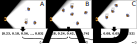
\includegraphics[width=0.9\linewidth]{figs/social-embeddings}
    \caption{In this example (and assuming the perspective of the yellow
    character), scenes A and B  are more related to each others (one person
    walking towards the character, with an independent group of people chatting
    in the background), than B and C (in C, the character is already engaged in
    an interaction).  Social embeddings make it possible to e.g. compare such
    social situations using a simple distance between vectors.}

    \label{fig:social-embeddings}
\end{figure}


Formally, if we denote $\mathcal{S}$ the set of social situations, the
\emph{social embedding} process has three steps: (1) a \emph{descriptor
extraction} step $D : \mathcal{S} \to \{\mathcal{D}\}$, with $\mathcal{D}$ the
set of descriptors that can be used to characterise a given social situation
(for instance, relative distances between people, facial expressions, group
membership), its physical environment (e.g. objects, location) and its context
(e.g. current task); (2) a \emph{description} step $T: \{\mathcal{D}\}^k \to
\mathcal{P}$, with $\mathcal{P}$ the set of textual descriptions, that combines
descriptors over $k$ previous timesteps into a coherent text-based description
of the on-going social situation, also implementing pruning strategies to avoid
the combinatorial explosion of possible descriptors combinations; and (3) the
embedding process itself $E : \mathcal{P} \to [0;1]^n$, mapping the textual
description to its embedding, i.e.  a vector of dimension $n$. $E$ is
implemented as a deep neural network, pre-trained on large datasets of natural
language.

Anecdotal evidence shows that the current generation of off-the-shelf LLMs (for
instance, OpenAI GPT-4) already has strong abilities to reason directly on
low-level social signals (like facial action units) to infer the high-level
state of a social situation (for instance, whether the interaction between two
persons is going well). As such, I do not plan in \project to train from scratch
a large language model, and accordingly, the project's focus is not on the
acquisition of large datasets of social interaction. Instead, I will perform
model fine-tuning on social tasks, using several existing datasets of
interactions, as detailed below.


%
%The basic idea of \emph{social robots} refers to robots that are situated in a
%human social environment. In this context, we expect social robots to exhibit
%\emph{social situation awareness}, i.e. to appraise and maintain a model of the social
%situation in which they are embedded. Depending on the role of the robot, this
%might include understanding who is present, who is interacting with whom, which
%are the resulting groups,  what are the in-group roles,  etc.
%
%social situation awareness, as a socio-cognitive skill, is essential for the robot to e.g.
%act in a context-sensitive manner; reason and apply social norms (for instance,
%do not navigate in the middle of a group, or do not suddenly interrupt a
%conversation); or create proactive social agents (in order to acknowledge and
%respond to a human who would like to engage with the robot, the robot must first
%adequately model and recognise the corresponding social situation).

%This can only be achieved if robots are endowed with the ability to represent
%not only their physical environment, but also their social environment and
%context. The \project project aims at designing, implementing and characterising
%a radically novel method to achieve this goal, based on the concept of
%\emph{embedding}: a low-dimensional, semantics-preserving, mathematical
%representation of a high-dimensional input (Figure~\ref{fig:social-embeddings}).
%Starting from a proof-of-concept of \emph{social embeddings} that I recently
%published~\cite{lemaignan2024social}, \project develops and fully characterise
%the concept of \emph{social embeddings}, that applies, for the first time, the
%idea of building a compact numerical representation to the complexity of social
%interactions and social dynamics.


%
%At a scientific level, 
%\TODO{articulate scientific impact}
%
%Finally, \project is also about asserting and reinforcing the European
%leadership in AI and intelligent robotics, in line with EU strong societal
%values: a physical AI system able to represent and reason about its social
%environment is also a system that can be designed to have an acceptable and
%positive social impact, in line with the European objectives for socially
%responsible AI. \project can directly contribute to these goals: the science and
%technology that underpins the project \textbf{provide an important contribution
%in securing a safe and responsible digital future in Europe}, as well as
%\textbf{\project building the capacity in Europe to develop socially intelligent
%embodied AI systems}. 

\subsection{Research objectives}

%\project is built around three axes: a basic research programme; an experimental
%programme that looks specifically at the application of social embeddings to
%social robotics; and, running in parallel to those first two axes, a scientific
%investigation of the ethical dimension of social embeddings.

This idea of \emph{social embeddings} builds on a proof-of-concept that I
validated in~\cite{lemaignan2024social}. \project will turn that early concept
into a mature mathematical tool for social sciences and artificial social
agents. As I explain below, I will formalize their construction,  fully
characterise their properties, expand their scope to complex, real-world social
situations, and demonstrate their transformative potential through deployment of
socially intelligent robots in multiple experimental settings.

\vspace{1em}

\noindent At the basic research level, \project targets two overarching research goals:

\begin{enumerate}[label=\textbf{(\arabic*)}]
    \item to build compact, yet semantics-preserving, embeddings to represent
arbitrary social situations; and to fully characterize these embeddings,
including their latent semantics. I translate this first goal into objective
{\bf O1}:

\begin{enumerate}[label=\textbf{O\arabic*}]
    \item \label{O1} To \textbf{construct and characterize the fundamental
properties of social embeddings}.
\end{enumerate}

    \item to precisely \textbf{define and implement the socio-cognitive skill of
        \emph{social sitation awareness} enabled by social embeddings}. I split this
        second goal into three specific objectives: \emph{social appraisal},
        \emph{social prediction}, \emph{social learning}.

\begin{enumerate}[label=\textbf{O2.\arabic*}]
    \item \label{O2.1} To use social embeddings to \textbf{automatically appraise
        social situations}, taking into account their \textbf{context}. Using
        a set of prototypical reference situations~\cite{kelley2003atlas}, social embeddings
        can be used to relate the current social situation to known ones.
        Besides, because social embeddings lend themselves to jointly encode
        social context by simply attaching context descriptions, the appraisal
        of the social situation can be made \emph{context-aware};

    \item \label{O2.2} To use social embeddings to model \textbf{social
        dynamics} by characterizing the trajectories of on-going social situations in the
        embedding space. I will look in particular into trajectories'
        \emph{discontinuties}, that might represent unexpected changes of social
        dynamics, and trajectories' \emph{extrapolations}, that might represent
        \textbf{social situation \emph{predictions}}.

    \item \label{O2.3} To \textbf{learn socially-appropriate behaviours} by using
        social embeddings as an additional input feature to existing robot behaviour
        generation algorithms, and by augmenting existing interactive machine
        learning techniques (`user in-the-loop' social learning for robots, that I
        pioneered in e.g.~\cite{winkle2021leador}) with
        representations of the social situation;

\end{enumerate}
\end{enumerate}

\noindent To illustrate these objectives, let consider the following imaginary
scenario: a robot is welcoming visitors at the entrance of an hospital; a group
of 3 persons are discussing together; one person is standing in the middle of
the room, glancing around; one last person is entering the hospital and
walks toward the reception. \ref{O2.1} will show that social embeddings can
represent and appraise this situation, accounting for the `hospital entrance' context: while
the person walking towards the reception probably does not need help from the
robot, the one in the middle seems uncertain, and might appreciate a pro-active
helping behaviour from the robot. \ref{O2.2} adds the temporal dimension: if we
sample the scene at regular time steps, and build a sequence of social
embeddings, what trajectory do they follow in the embedding space? Is it
continuous? Is there any rapid changes? Can we extrapolate this trajectory to
predict where the situation is going? \ref{O2.3}, finally, looks at exploiting
social embeddings for socially-aware behaviour learning. In our scenario, a
member of the hospital staff would for instance teach the robot an
context-appropriate response, and the robot would be able to generalise it to
other, similar social situations.


I want to evidence these properties in both lab-based experiments and
real-world deployments on social robots. Accordingly, \project has two addtional
objectives:

\begin{enumerate}[label=\textbf{O\arabic*}]
    \setcounter{enumi}{2}
    \item \label{O3} To fully {\bf integrate social embeddings onto a
        socio-cognitive architecture for autonomous service robots} and,

    \item \label{O4} To conduct an {\bf ambitious experimental programme},
        including both lab-based and field research, to demonstrate the
        effectiveness of social embeddings in complex, real world conditions.
        This means deploying the \project robot into existing social eco-systems
        that are sufficiently complex, yet open to explore novel social interactions.
\end{enumerate}


%Once completed, these four objectives will provide solid theoretical and
%empirical foundations to social embeddings.
%
%Each of these four objectives involve both basic and experimental research,
%presented in the next section.


%%%%%%%%%%%%%%%%%%%%%%%%%%%%%%%%%%%%%%%%%%%%%%%%%%%%%%%%%%%%%%%%%%%%%%%%%%%%%%%

\section{Methodology and implementation}
%\section{Feasibility of the project}

\project delivers on its programme by combining a range of scientific methods.
Embedding-based data representation is the central method underpinning the
generation of social embeddings. From a computational point of view, it relies
on specialized deep learning models to generate the source descriptors, and
knowledge graph and propositional logic to combine descriptors into full text
descriptions. The selection of descriptors and their combination is however also
informed by social psychology and sociology, and I accordinlgy perform
qualitative field observations of social situations.

\TODO{make sure we have tasks for that}

The analysis of the resulting embeddings uses... \TODO{complete}

%machine learning large language models fine-tuning and embedding learning learning;
%user-centered design; ethnographic and sociological investigation; expressive
%non-verbal communication; embodied cognition; symbolic AI; neural nets and
%sub-symbolic AI; interactive machine learning.

In terms of implementation, the \project project work programme is organised in
four main work packages that I briefly outline hereafter, with the key research
methods that I will employ in each of them.

%The first one, \emph{\WPA}, focuses on basic research; the second
%one, \emph{\WPB}, focuses on the artificial socio-cognitive skills enabled by
%social embeddings; the third one, \emph{\WPC}, specifically look at the
%application and impact on social robots; and the final one, \emph{\WPD},
%organises the experimental work.

\TODO{list and explicitely name the employed methodologies}

\subsection{WP1: \textbf{\WPA}}

WP1 addresses Objective \textbf{O1}. I will first systematically investigate the
three steps of social embeddings construction, and then characterize the
resulting embeddings.

Social embeddings construction requires first to extract descriptors, then to
build complete textual descriptions, and finally to embed these descriptions.  I
will extract basic social descriptors using the ROS4HRI social perception
approach, as it formalize a multi-modal model of humans~\cite{lemaignan2022ros},
and run in real-time on current robots. I will augment these basic descriptors
with more complex percepts, including (1) descriptors of human-objects
interactions (HOI), using transformer-based techniques
like~\cite{iftekhar2022what} ; (2) affective
descriptors~\cite{vinciarelli2009social}, using e.g. facial expressions based on
facial action units classification~\cite{martinez2019automatic}; (3) group-level
interactions, including $f$-formations~\cite{setti2015fformation}, and group
activity recognition, using deep convolutional graph techniques like
ARG~\cite{wu2019learning}.

%(3) a novel contextual model of
%attention~\cite{ferrini2024percepts} that allows fine-grained assessment of what
%the person around the robot are focusing on.

The generation of textual descriptions consists in both the combination of
descriptors into textual \emph{snapshots} of the social environment at a
specific time, and the combination of these snapshots over time, to build a
textual description of complete situations with a time horizon of 10s to
25s~\cite{netanyahu2021phase}. I will initially build snapshots using text
templates, and then extend the methodology using techniques based on
social knowledge graphs~\cite{sap2019atomic} and propositional
logic~\cite{tsoi2022sean}. The combination of snapshots into social situations
will be developed with the help of the PHASE simulator and
dataset~\cite{netanyahu2021phase}, that includes a large number of annotated
social interaction sequences.

Last, the text embedding process itself. Due to the fast pace of progress in the
LLMs landscape, it is likely that current
methods (including e.g.~\cite{reimers2019sentencebert,muennighoff2022sgpt}) will
have been superseeded by new methods. I will closely monitor
advances in the domain, especially on the question of semantic
relatedness~\cite{thakur2021beir}, as this is critical for social
embeddings. I plan to perform fine-tuning~\cite{hadsell2006dimensionality}
of the selected text embedders to specialize them for social situation
representation. I will do so by leveraging existing open-access annotated
datasets of social interaction like AMI~\cite{carletta2007ami},
D64~\cite{oertel2013d64}, SALSA~\cite{alameda2015salsa}, or my own SoGrIn
dataset~\cite{webb2023sogrin}, and datasets of social questions-answers like
SocialIQa~\cite{sap2019social}.

I will then characterise social embeddings, starting with the fundamental
properties that I identified in~\cite{lemaignan2024social}: invariance to
syntax, social similarity and continuity. Next, and of particular interest, is
the characterization of the embeddings' \emph{latent semantics}: For instance,
social descriptions like `two persons chatting and laughing
together'; or `a group of three people walking together'; or `one single person
walking towards the robot, looking agitated'; etc.  are all semantically
distinct, and, consequently, would belong to distinct regions in the embedding
space. Identifying such clusters to characterize the semantic topology of the
embedding space~\cite{sun2023topological} will be achieved by exploiting
existing annotated datasets to identify and extract prototypical reference social situations.

\vspace{1em}
\noindent\emph{ Timeframe: Y1-Y3; one post-doc (PD1) with expertise in
    deep learning/text embedding; one post-doc (PD2) in data-driven sociology.}


\subsection{WP2: \textbf{\WPB}} 

Work package WP2 focuses on research objectives \ref{O2.1}, \ref{O2.2} and \ref{O2.3}:
expanding social embeddings beyond their fundamental properties, to build a
`social situation awareness' cognitive skill for social robots.

%\emph{social situation awareness} is a socio-cognitive skill that is essential for
%artificial social system, like social robots, to e.g.  act in a
%context-sensitive manner, reason and apply social norms,
%or create proactive social agents (in order to acknowledge and respond to a
%human who would like to engage with the robot, the robot must first adequately
%model and recognise the corresponding social situation).


% METHODS for the 3 objectives?
%- appraise social situations, also taking into account the social context
%- learn socially-appropriate behaviours
%- anticipate future social states


Social appraisal (Objective~\ref{O2.1}) is about interpreting the results of WP1
in terms of social situations. This includes, in particular, mapping regions of
the embedding space to known social situations, as identified for instance
in~\cite{kelley2003atlas}. \TODO{complete}

Context-awareness is another critical aspect of social situation appraisal.
\emph{Context} has been defined in various way, including as \emph{who},
\emph{what}, \emph{when}, \emph{where}, and \emph{why} of
interactions~\cite{vinciarelli2009social}; as high-level task/environment
characteristics, such as `studying' or `dining'~\cite{nigam2015social}; as
relationships between agents in the scene, such as `interacting in a group',
`standing in a line'~\cite{althaus2004navigation}; or as
task-based~\cite{castellano2012detecting}. Social embeddings lend themselves
well to context encoding: as long as a context description can be generated, it
can be appended to the social situation description, and jointly embedded.

%\emph{Characterizing} how context impacts the resulting social embeddings
%requires extensive research, from defining and specifying a taxonomy of
%contexts, to characterizing their impact on the social embedding space.


Objective~\ref{O2.3} is about analysing \emph{social dynamics} by
studying the \emph{trajectories} of social situations in the embedding space.
For instance, the velocity in the embedding space should reflect the rate of
change of a social situation in the physical space; trajectory extrapolation
could be employed by robots to anticipate upcoming social situations;
discontinuities in the embedding space would reflect brutal social changes that
could trigger specific robot behaviours (for instance to acknowledge or attempt
to repair social situations).
\TODO{need to be SMART: reference specific techniques + metrics}

Objective~\ref{O2.3}, finally, looks at the learning of socially-appropriate
behaviour generation. \project aims at significantly advancing the state of the
art in this regard, by combining two techniques: (1) machine learning-based
generation of affective robot motion, using either generative neural
networks~\cite{marmpena2019generating,suguitan2020moveae} or reinforcement
learning~\TODO{cite?}; (2) interactive machine learning in high-dimensional
input/output spaces, where I have shown with my students promising results for
generating complex social behaviours~\cite{senft2019teaching, winkle2020couch}
that fully involve the end-users~\cite{winkle2018social}. Modulating (1) with
the social embedding of the current situation will enable the generation of
non-repetitive and socially appropriate behaviours (gestures, motions, gazing
behaviours, facial expressions); augmenting the input space of (2) with social
embeddings will enable the robot to learn contextualised social policies.


\vspace{1em}
\noindent\emph{Timeframe: Y1-Y4; one post-doc PD3 in cognitive sciences; one PhD student in data-driven sociology (PHD1)}

\subsection{WP3: \textbf{\WPC}}

This workpackage focus on the practical integration of social embeddings in a
larger cognitive architecture for autonomous social robots, and correspond to
Objective~\ref{O3}. It will effectively enable the experimental program of
\project.  In WP3, I will develop the required perceptual and behavioural
capabilities of the robot, implement the real-time generation of social
embeddings, and integrate together a principled socially-aware robot supervisor,
that exploits social embeddings.

\begin{wrapfigure}[11]{l}{0.15\linewidth}
    \centering
    \vspace{-10pt}
    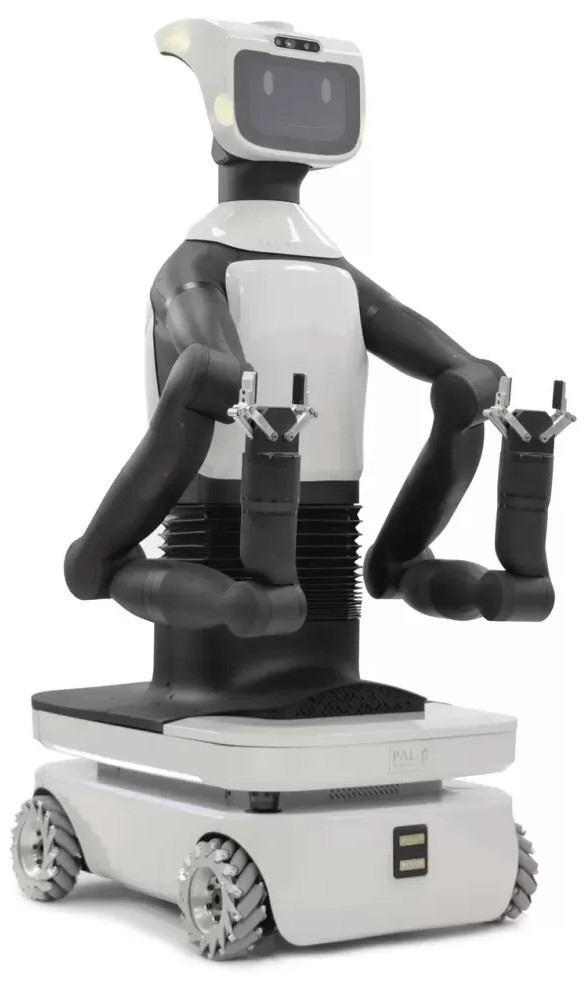
\includegraphics[width=\linewidth]{tiagopro}
    \label{fig:tiagopro}
\end{wrapfigure}

As \project focuses specifically on the AI engine of the robot, I will use an
existing off-the-shelf social robot, a PAL Robotics TIAGoPro
(pictured on the left). TIAGoPro offers out-of-the-box advanced human perception
based on the ROS4HRI framework (that I myself originally
designed~\cite{mohamed2021ros4hri} as an international standard for Human-Robot
Interaction~\cite{lemaignan2022ros}). It also offers on-board GPU options that
are appropriate to implement a fully AI-based autonomous system. I have
extensive experience with this platform, having actually directly taken part to
its design and software stack implementation while employed at PAL Robotics.

I will be using publicly available resources, including machine
learning backbones and state-of-art open-source
pre-trained Large Language Models (foundational models) like
Llama2~\cite{touvron2023llama}; I have shown in~\cite{lemaignan2024social} that
simple social embeddings can indeed already be generated in near-real time on
consumer-grade GPUs. The integration of social embeddings in a larger cognitive
architecture suitable for social robots will require extending existing
robotic architectures, of which I have extensive
experience~\cite{lemaignan2017artificial, lemaignan2015pyrobots,lemaignan2011what}.

\vspace{1em}
\noindent\emph{Timeframe: Y2-Y5; one PhD student (PHD2) in cognitive robotics.}

\subsection{WP4: \textbf{\WPD}}

Finally, WP4 organises the experimental work, and aim at achieving~\ref{O4}. I
intent to run both controlled experiments in lab settings to evidence the basic
properties of social embeddings, their translation in terms of social situation awareness,
as well as more complex deployments in real-world, naturalistic settings, to
demonstrate how social embeddings might push the boundaries of social
intelligence for service robots.

As an example of controlled experiment, I will adapt to social
robotics~\cite{lemaignan2015mutual} experimental protocols originally designed
by Frith and Happé~\cite{frith1994autism} to investigate social representation
and mental modelling in autistic children. This protocol include tasks like
distinguishing \emph{happiness} or \emph{sadness} from \emph{surprise}, or
distinguishing \emph{sabotage} from \emph{deception}: these nuances, quite
self-explanatory to experienced social agents, require subtle modelling of the
context and mental state of agents, and, until now, have not been successfully
reproduced on robots. I aim to show that social embeddings offer a generic
methodology to implement this kind of advanced social understanding.

Real-world studies, on the other hand, will be conducted in collaboration with
the Broca hospital, a geriatic hospital with a strong track record of
experimentation with robots and dedicated facilities.  Building on my
fieldwork
experience
(e.g.~\cite{hood2015when,mondada2015ranger,winkle2018social,cooper2023challenges}),
and my on-going collaboration with Pr. Pino, coordinator of the Broca Living Lab, I will
deploy an autonomous social robot for several weeks, using social embeddings to
implement a level of social situation awareness and social appropriateness not yet
achieved in this type of application.

\vspace{1em}
\noindent\emph{Timeframe: Y1-Y5; with involvement of the whole research team}

%
%My extensive track-record of fieldwork and real-world robot deployments (in a
%broad range of environments, including schools~\cite{hood2015when,
%lemaignan2016learning, jacq2016building,
%baxter2015wider,kennedy2016cautious,senft2018robots,lemaignan2022social}, at
%people's home~\cite{mondada2015ranger}, in public
%spaces~\cite{alhafnawi2022deliberative}, or in healthcare
%environments~\cite{winkle2020couch,cooper2023challenges}).
%
%
%\TODO{need to be SMART: reference specific techniques + metrics}

%
%\subsection{Additional workpackages}
%
%Because the development of socially-intelligent robots has
%complex ethical ramifications -- including the potential of alienating
%human users, \project also includes an explicit research component on
%Responsible Robotics. In particular, the project will aim to contribute directly
%to the on-going roadmap for Responsible Robotics, specifically
%investigating the interplay between social embeddings, transparency and human
%agency. The work will be conducted in workpackage WP4.

%
%Social embeddings, by enabling artificial systems to model and reason on their
%social environment, have the potential of significantly increase the social
%competencies of e.g. robots, also raising ethical questions.
%
%I am part of an international working group on Responsible Robotics~\TODO{cite
%Dagsthul roadmap arxiv}...
%
%WP6 aims at establishing the conceptual and ethical framework around the idea of
%\emph{robot-supported human-human interactions}. It does so by co-creating
%patterns of interaction and norms with the general public, using a unique
%combination of ethnographic observations and `crowd-sourced' interaction
%patterns.
%
%\vspace{1em}
%\noindent\emph{Timeframe: Y3-Y5; one senior post-doc (PD3)
%with background in ethics of technology and responsible innovation.}



%
%A final workpackage WP5 groups all the task related to the grant management, as
%well as the dissemination and exploitation tasks. Details of the dissemination
%and exploitation activities are provided in Part B2 of the proposal.

%%%%%%%%%%%%%%%%%%%%%%%%%%%%%%%%%%%%%%%%%%%%%%%%%%%%%%%%%%%%%%%%%%%%%%%%%%%%%%%%%%%%
%%%%%%%%%%%%%%%%%%%%%%%%%%%%%%%%%%%%%%%%%%%%%%%%%%%%%%%%%%%%%%%%%%%%%%%%%%%%%%%%%%%%
%%%%%%%%%%%%%%%%%%%%%%%%%%%%%%%%%%%%%%%%%%%%%%%%%%%%%%%%%%%%%%%%%%%%%%%%%%%%%%%%%%%%

\section{Ambition of the \project project}

\TODO{rephrase + clarify what goes in this section}

Social robots are emerging as key enablers to address several
emerging societal challenges, like the ageing society or increasing social
isolation. In this context, not only we lack appropriate tools to model the
social environment of robots, severely limiting their effectiveness, but also
researchers in social robotics have the prime responsibility to ensure that
robots can properly understand and reason about their spatial and social
environment, also ensuring responsible and positive societal impact. As such,
beyond using robots as an experimental methodology, \project also has the
ambition to significantly transform the field of social robotics itself.


\newpage

\printbibliography



%\vspace{0.5em}
%\begin{itemize}
%
%    \item What are the conceptual, algorithmic and technical prerequisites to
%        design and implement such an autonomous \& responsible robots? in
%        particular, what social context understanding and (machine) learning
%        architectures are required to \textbf{enable long-term autonomy} and,
%        eventually, \textbf{engagement} between a robot and its end-users?
%
%    \item What are the conditions and methodologies enabling large scale data
%        acquisition of \textbf{real world, user-driven robots behaviours}? How
%        to then train robots to become \textbf{progressively autonomous}?  And
%        ultimately, how to balance \textbf{autonomy} of the robot with the
%        necessary \textbf{behaviour transparency} and \textbf{human oversight}?
%
%    \item What are the public expectations with respect to the role of social
%        robots, and how can we \textbf{collaboratively design}
%        \textbf{autonomous}, yet \textbf{responsible, beneficial, socially
%        acceptable robots}?
%
%\end{itemize}
%
%\vspace{0.5em}
%\noindent From these questions, I derive the following four objectives that are
%the guiding principles of my research program, both in the short term, and at a
%10-15 years horizon:


%\subsection{Work plan outlook}
%
%My research program could begin rapidly, using publicly available resources,
%including machine learning architectures like Transformers, combined with open-source
%pre-trained Large Language Model backbones; and state-of-art HRI tools like
%ROS4HRI~\autocite{mohamed2021ros4hri} to represent in real-time the social
%environment of the robot. While long and complex data collection campaigns would
%have to be organised, and training infrastructure would need to
%be designed, I expect initial results in the first 3 to 5 years.
%
%This is also a long-term vision: on the one hand, the rapid pace of progress
%of technology (novel deep machine learning architectures, novel HRI tools for
%human and scene understanding) continuously opens novel investigation
%venues; one the other hand, the success of my research vision hinges on
%real-world, long-term experimental work: deploying robots in the healthcare
%sector, creating the conditions for adoption by the end-users, running
%long-term deployments with the end-users are long terms aims
%,... these research activities will take
%place over long period of time.

%\subsection{Importance and impact}
%
%My research program has the potential to be groundbreaking: until now,
%autonomous social robots have had little real world success. Experiments and
%deployments have been mostly limited to constrained application domains, where
%rigid action policies (scripts, task planners) could be sufficient. State-of-art
%robots however fail to handle the complexity and unpredictability of real world
%environments (like the ones encountered in the healthcare domain). In addition,
%these systems see poor field adoption due to several factors including
%difficulty of use, wrong expectations, perceived complexity.
%
%This research program is also important: as socially assistive robots quickly
%develop, it is critical to equip ourselves with a deeper understanding and
%intellectual framing of what social robots \emph{could} and \emph{should} be,
%paving the way for their much broader adoption in the coming years: I will
%actively contribute to this aim, by leading the design and implementation of
%socially-intelligent robots that are socially useful, acceptable in the
%long-term, and ethically responsible, but also by furthering my engagement to
%interdisciplinary work, and broad engagement with the society and policy makers.







%%%%%%%%%%%%%%%%%%%%%%%%%%%%%%%%%%%%%%%%%%%%%%%%%%%%%%%%%%%%%%%%%%%%%%%%%




%How this general
%principle translates into specific guidelines and algorithms -- while taking into
%account the principles of a responsible AI -- is the central
%contribution of Work Package 1.

% This socially-driven goal forms what we call a \emph{social
%teleology}. its own goals have this objective can only be achieved if the
%robot is \textbf{socially-driven}: the robot's behaviours must be driven by the
%intention to support positive human-human interactions. 


%I frame these hypotheses with the idea of \textbf{robot-supported human-human
%interactions}, a novel conceptual framework to `think' the future human-robot
%interactions. I will co-construct this framework through large scale public
%engagement: for a whole year, I will deploy the \project robot within the City
%Lab of Bristol's science centre \emph{WeTheCurious}, relinquishing the control
%of the robot to the visitors themselves. Tasked with remotely operating the
%robot to assist fellow visitors, I will accompany them in `inventing by doing' a
%new grammar of social interactions: what does it mean for a robot to help? How
%to do so in the dynamic, messy, environment of a science centre? What are acceptable
%behaviours? Can we see new social norms emerge? At the end of this experiment,
%we expect 1000s of people to have had experienced -- and co-designed -- how
%robots should interact with humans in a positive, helpful way, and each of these
%experiences will contribute to uncovering and designing the basic principles of
%social interaction for robots. This work is the focus of WP1.
%
%While most of the interactions in the science centre will be short-lived, two further
%large scale experiments will take place over the course of the project: a
%one-year experiment in one of Bristol's Special Education Needs (SEN) school,
%helping 250+ children with psycho-social impairments to develop their social
%skills; a second one-year experiment at the Bristol's children hospital, where
%the robot will join one of the wards where 30+ children with long-term conditions
%stay for months, and engage with the children into playful social activities: telling
%stories, triggering group activities with other children, providing additional
%social presence. In both these experiments, the robot behaviours will be
%co-designed with, and learnt from the end-users themselves: nurses, teachers,
%parents, and where possible, the children themselves.
%
%
%\section{Overview of the \project work programme}
%
%Socially intelligent robots require unique, beyond state-of-the-art,
%capabilities to \emph{(1)} understand the social interactions (social
%situation awareness), \emph{(2)} autonomously decide the best course of action for
%short-term and longer-term social influence, and \emph{(3)} perform the
%appropriate social actions and exert said influence in an appropriate,
%responsible manner.
%
%Not only the required technology is itself beyond state-of-the-art (and will be
%researched and integrated in WP2, WP3 and WP4), but the
%interplay between technology, socio-cognitive psychology, privacy and ethics is
%only starting to be researched and understood. \project offers an
%strong vision and an ambitious, evidenced-based, methodology to significantly
%advance our understanding of this multi-faceted problem.
%
%
%\begin{itemize}
%    \item \textbf{O1: conceptual framing} To construct a solid conceptual
%        framing around the multidisciplinary question of responsible human-robot
%        interactions, answering questions like: What should motivate the robot
%        to step in and attempt to help? or: What social norms are applicable to
%        the robot behaviours? Building on the extensive body of work on
%        Responsible AI, I will investigate the basic principles of
%        responsible robot-mediated social interactions, that must form the
%        foundations of a socially useful robot, accepted and used in the long
%        run.  Using user-centred design and participatory design methodologies,
%        I will identify the determinants and parameters of a responsible social
%        intervention, performed by a socially-driven robot, and formalise them
%        in practical principles.
%
%    \item \textbf{O2: physical-social representation and reasoning} To
%        effectively and responsibly interact with its environment, the robot
%        must first build a comprehensive and continuously updated model, from its
%        spatial and physical configuration, to its social dynamics. I will
%        design and develop a novel cognitive capability of artificial
%        \emph{social situation assessment} to enable the robot to represent
%        real-time social dynamics in its environment. I will achieve this
%        breakthrough by combining existing model-based approaches \TODO{refs}
%        (including my recent research on social state modeling \TODO{refs}, with
%        the expressive power of the new \emph{social embeddings} that I have
%        recently introduced.
%
%    \item {\bf O3: goal-driven, responsible decision making} I aim to create
%        robot behaviours that are perceived as purposeful and intentional
%        (long-term goals), while being shaped by a user-created and
%        user-controlled action policy.  I will integrate long-term social goals,
%        arising from the interaction principles of \textbf{O1}, with the social
%        modeling capability of \textbf{O2}, into a principled, goal-driven
%        cognitive architecture, with responsible AI guarantees. The breakthrough
%        will come from combining these long-term social goals with bottom-up
%        action policies, designed and learnt from the end-users using
%        human-in-the-loop attention-based machine learning.
%
%        I want to specifically test the following two hypotheses: first, that
%        long-term social goals, if suitably co-designed with the public and
%        stakeholders and properly integrated into the robot as a \emph{social
%        teleology}, will create the perception that the robot is intentional and
%        purposeful. This will in turn elicit sustained engagement from its human
%        users.
%
%        Second, that human-in-the-loop machine learning can be used to ensure an
%        additional layer of human oversight and a level of behavioural
%        transparency.  Human-in-the-loop reinforcement learning -- as
%        implemented in the SPARC approach that I have developed with my students
%        and already used in complex social
%        environments~\parencite{senft2017supervised,senft2019teaching,winkle2020insitu}
%        -- relies on an end-user `teacher'. This teacher initially fully
%        controls the robot (via teleoperation) while it learns the action
%        policy, and then progressively relinquishes control up to a point where
%        the robot is effectively autonomous. As I previsouly argued
%        in~\textcite{senft2019teaching}, this approach leads to increased
%        control and ownership of the system, and as a result, increased trust
%        from the end-users.
%
%
%    \item{\bf O4: ambitious field research} Finally, the last major objective of
%        my research project is to demonstrate the effectiveness of my approach
%        in complex, real-world conditions. This means deploying the socially
%        interactive robots in existing social \emph{ecosystems} that are
%        sufficiently complex and open to explore novel social interactions. My
%        objective is also to show that this real-world deployment can be
%        successfully driven by the `end-to-end' involvement of all the end-users
%        and stakeholders: from defining the robot's role, from the different
%        perspective of each end-user, to actually designing and `teaching' the
%        robot what to do.
%
%
%\end{itemize}




%%%%%%%%%%%%%%%%%%%%%%%%%%%%%%%%%%%%%%%%%%%%%%%%%%%%%%%%%%%%%%%%%%%%%%%%%%%%%
%%%%%%%%%%%%%%%%%%%%%%%%%%%%%%%%%%%%%%%%%%%%%%%%%%%%%%%%%%%%%%%%%%%%%%%%%%%%%
%%%%%%%%%%%%%%%%%%%%%%%%%%%%%%%%%%%%%%%%%%%%%%%%%%%%%%%%%%%%%%%%%%%%%%%%%%%%%

%\newpage
%
\chapter{B1.b Curriculum-vitae and track record}\label{the-principal-investigator}

%\eu{should follow the suggested template. Include any career
%breaks or unconventional career paths, so that your career stage is fairly assessed by the evaluation
%panels. You should as well list your current grants and on-going and submitted grant applications in
%the funding ID table (this table will not count towards the page limits).}
%\eu{(max 2 pages)}

{\LARGE \bf Dr. Séverin Lemaignan}

\vspace{2em}

\section{Personal details}

\begin{tabular}{p{0.45\linewidth}p{0.45\linewidth}}
    \textbf{ORCID}:
    \href{http://orcid.org/0000-0002-3391-8876}{0000-0002-3391-8876} & \textbf{Date of birth}: 17 Jan 1983 (37 years old) \\
\textbf{Nationality}: French & \href{https://academia.skadge.org}{academia.skadge.org} -- \href{https://twitter.com/skadge}{twitter.com/skadge}
\end{tabular}

\vspace{2em}

\subsection{Education and key qualifications}

\begin{tabular}{p{0.15\linewidth}p{0.8\linewidth}}
    \bf 2008 -- 2012 & {\bf Joint German-French PhD in Cognitive Robotics}
    \newline LAAS-CNRS, France / Technical University of Munich, Germany
    \newline {\small Supervisors: Pr. Rachid Alami, CNRS; Pr. Michael Beetz,
    TUM} \\
    \bf 2004 -- 2005 &  {\bf MSc Artificial Intelligence for Learning
    Technologies}
    \newline University Paris V, France \\
    \bf 2002 -- 2002 & {\bf Joint German-French MSc of Engineering} \newline Karlsruhe
    Institute of Technology, Germany / ENSAM ParisTech, France \\
\end{tabular}

\subsection{Current position}

\begin{tabular}{p{0.15\linewidth}p{0.8\linewidth}}
    \bf 2021 -- & {\bf Head of Social Robotics and HRI Research}
    \newline PAL Robotics, Barcelona, Spain 
    \newline \small Head of the Human-Robot Interaction research and enginerring
    group.\\
\end{tabular}


\subsection{Previous positions}

\begin{tabular}{p{0.15\linewidth}p{0.8\linewidth}}
    \bf 2019 -- 2021 & {\bf Associate Professor in Social Robotics and Artificial
    Intelligence}
    \newline Bristol Robotics Laboratory, University of the West of England,
    United Kingdom 
    \newline \small Head of the Human-Robot Interaction research group; Head of the Driverless Vehicle research group.
Directly managing 20+ students and early career researchers. \\
    \bf 2018 -- 2019 & {\bf Senior Research Fellow in Robotics and AI} \newline Bristol Robotics Laboratory, University of the West of England, United Kingdom \\
    \bf 2017 -- 2018 & {\bf Lecturer in Robotics} \newline Plymouth University, Plymouth, United Kingdom \\
    \bf 2015 -- 2017 & {\bf EU Marie Skłodowska-Curie Post-doctoral fellow}
    \newline Plymouth University, Plymouth, United Kingdom \newline \small
    Development and Implementation of a Theory of Mind for robots \\
    \bf 2013 -- 2015 & {\bf Post-doctoral fellow} \newline CHILI, EPFL,
    Lausanne, Switzerland \newline \small Interaction with Robots in Learning
    Environments – Supervision of the robotic group \\
    \bf 2012 -- 2013 & {\bf Post-doctoral fellow} \newline LAAS-CNRS, Toulouse,
    France \newline \small Spatial and Temporal Reasoning for Cognitive Robotic
    Architectures\\
    \bf 2006 -- 2007 & {\bf Research Engineer} \newline INRIA, Paris, France
    \newline \small Development of semantic-aware control architectures for
    autonomous vehicles \\
\end{tabular}


\section{RESEARCH ACHIEVEMENTS AND PEER RECOGNITION}

\subsection{Research achievements}

%\resizebox{\linewidth}{!}{
\hspace*{-0.5cm}\begin{tabular}{p{1.7cm}p{7cm}p{8cm}}

    \vspace{-0.2cm}
\includegraphics[height=2.2cm]{thumbs/2019-science.png} & Senft, E.,
    \ul{Lemaignan, S.}, Baxter, P., Bartlett, M., Belpaeme, T.
    \newline\href{https://doi.org/10.1126/scirobotics.aat1186}{\textbf{Teaching robots
    social autonomy from in situ human guidance}}
    \newline \textit{Science Robotics} 2019
    & \small A novel human-in-the-loop machine learning approach
    to implement social autonomy in a robot, with several deployments in UK
    public schools. This is a first-in-kind demonstration of learning autonomous
    action policy in a high dimensional, socially complex,
    environment.\textbf{\newline[main study supervisor]} \\


    \vspace{-.20cm}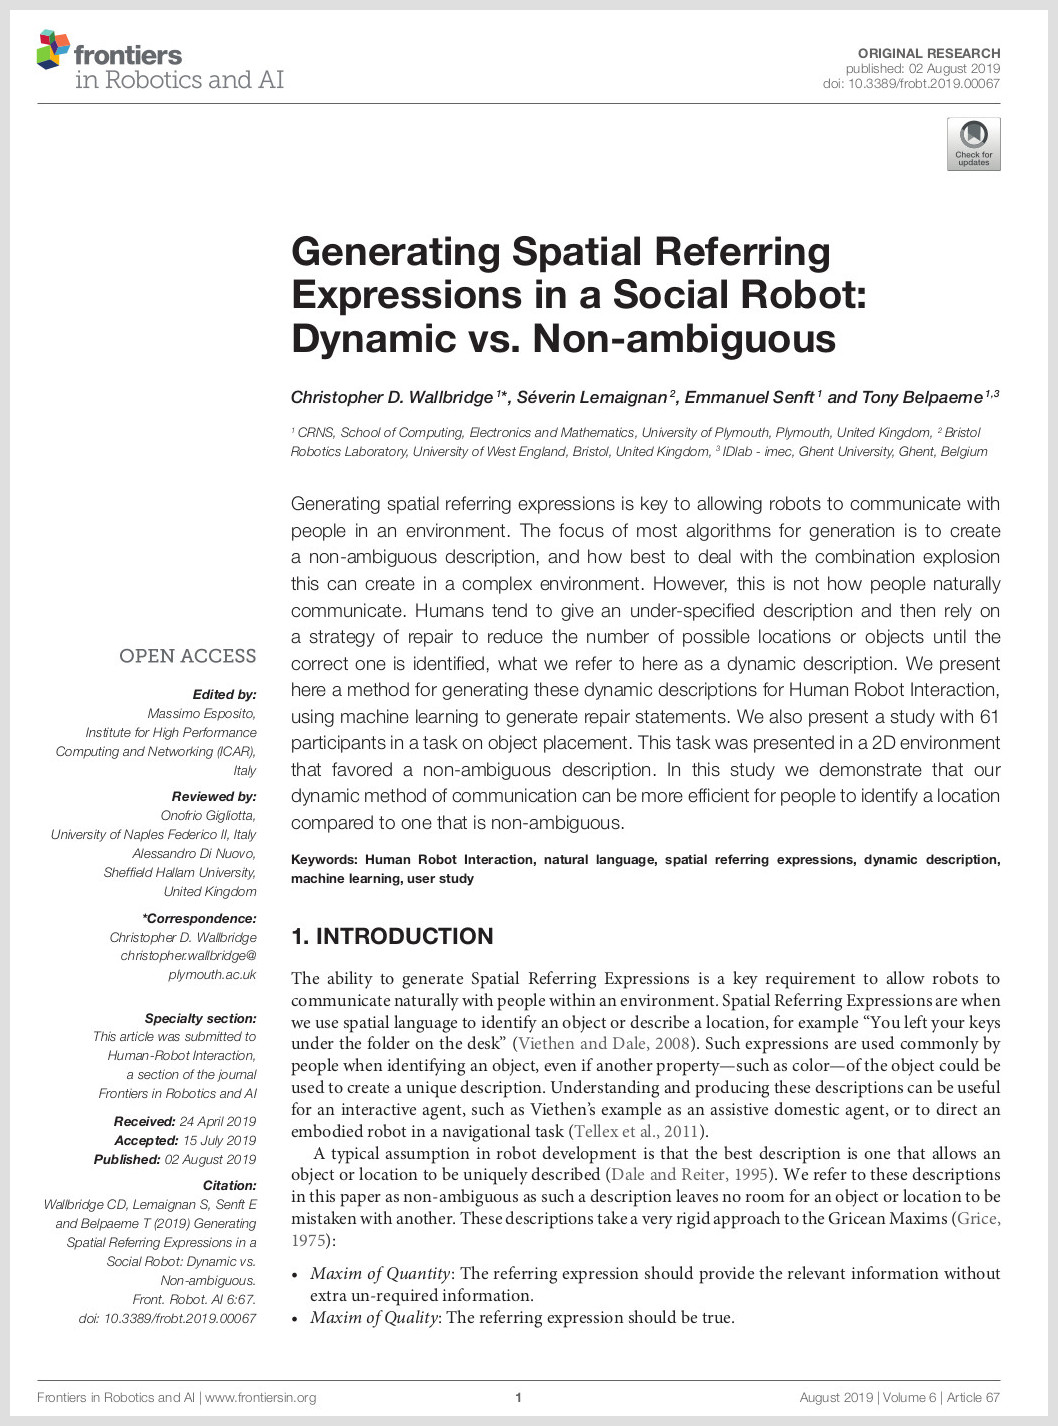
\includegraphics[height=2.2cm]{thumbs/2019-frontiers-chris.jpg} &

    Wallbridge, C., \ul{Lemaignan, S.}, Senft, E., Belpaeme, T.  
    \newline\href{https://doi.org/10.3389/frobt.2019.00067}{\textbf{Generating
    Spatial Referring Expressions in a Social Robot: Dynamic vs Non-Ambiguous}}
    \newline \textit{Frontiers in AI and Robotics} 2019
    & \small Challenges the common understanding that robots should be
    unambiguous: we show that ambiguity is often desirable for fluid and natural
    human-robot interactions.\textbf{\newline[main study supervisor]}  \\

    \vspace{-.20cm}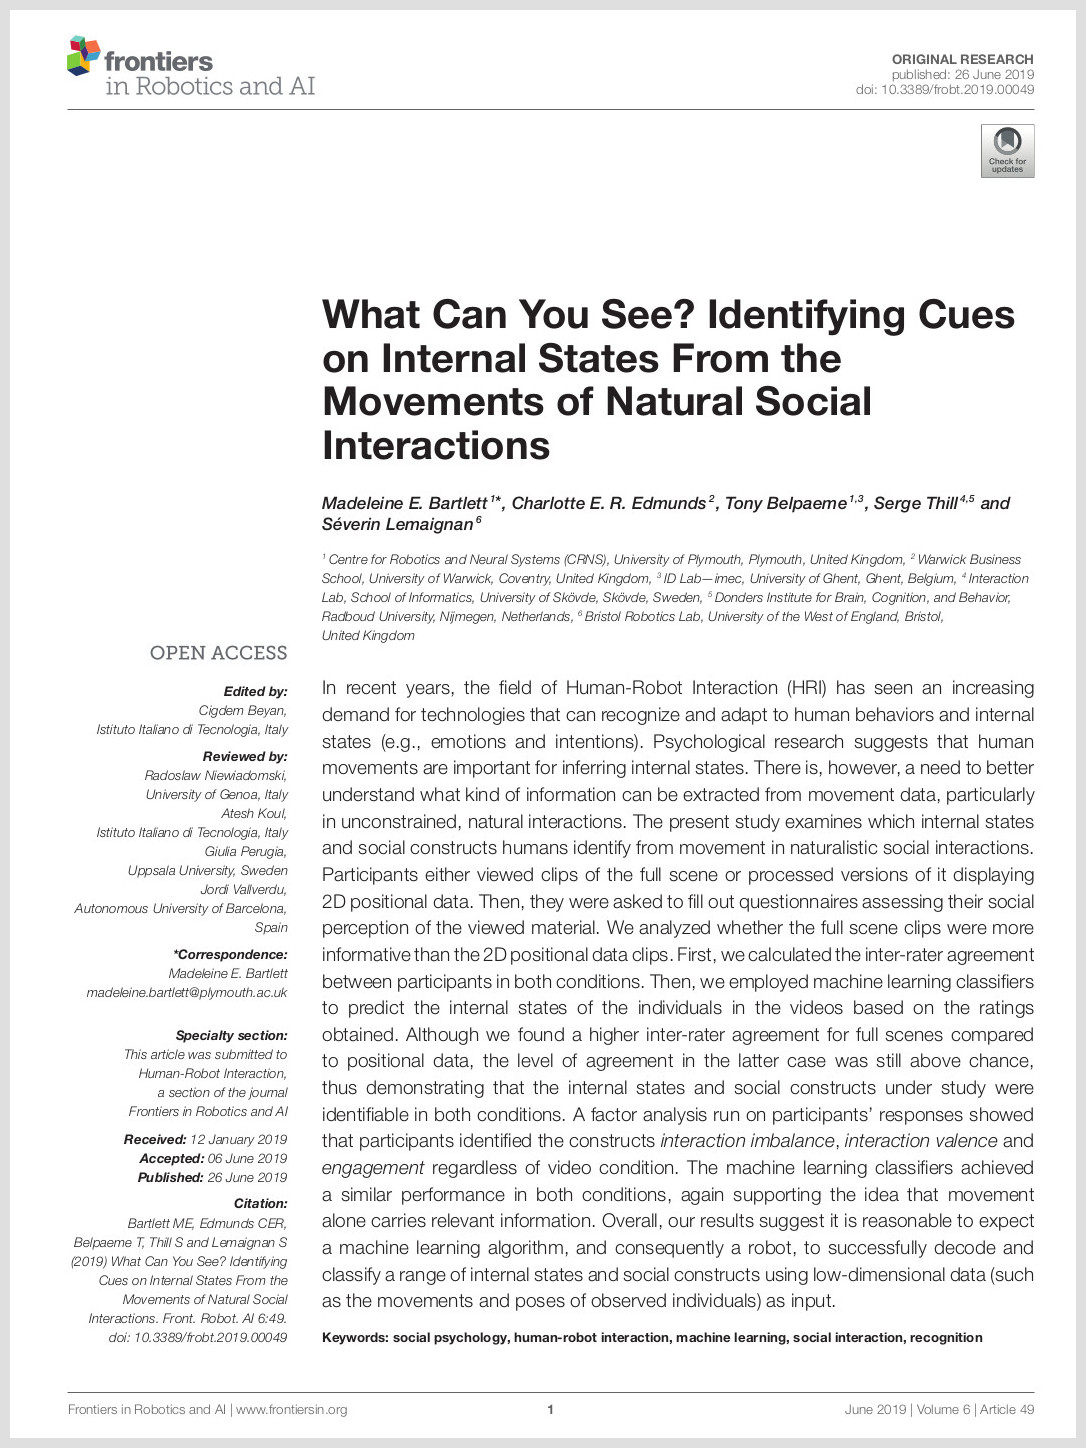
\includegraphics[height=2.2cm]{thumbs/2019-frontiers-maddy.jpg} &

    Bartlett, M., Edmunds, C. E. R., Belpaeme, T., Thill, S., \ul{Lemaignan, S.} 
    \href{https://doi.org/10.3389/frobt.2019.00049}{\textbf{What Can You See? Identifying Cues on Internal States from the
    Kinematics of Natural Social Interactions}} 
    \newline \textit{Frontiers in AI and Robotics} 2019
    & \small Investigates how partially hidden 'internal states' (like emotions,
    cooperativeness, etc) can be decoded from simple visible cues, like
    skeletons. Also demonstrates that social situations can be described along 3
    simple dimensions.\textbf{\newline[main study supervisor]}\\


    \vspace{-.20cm}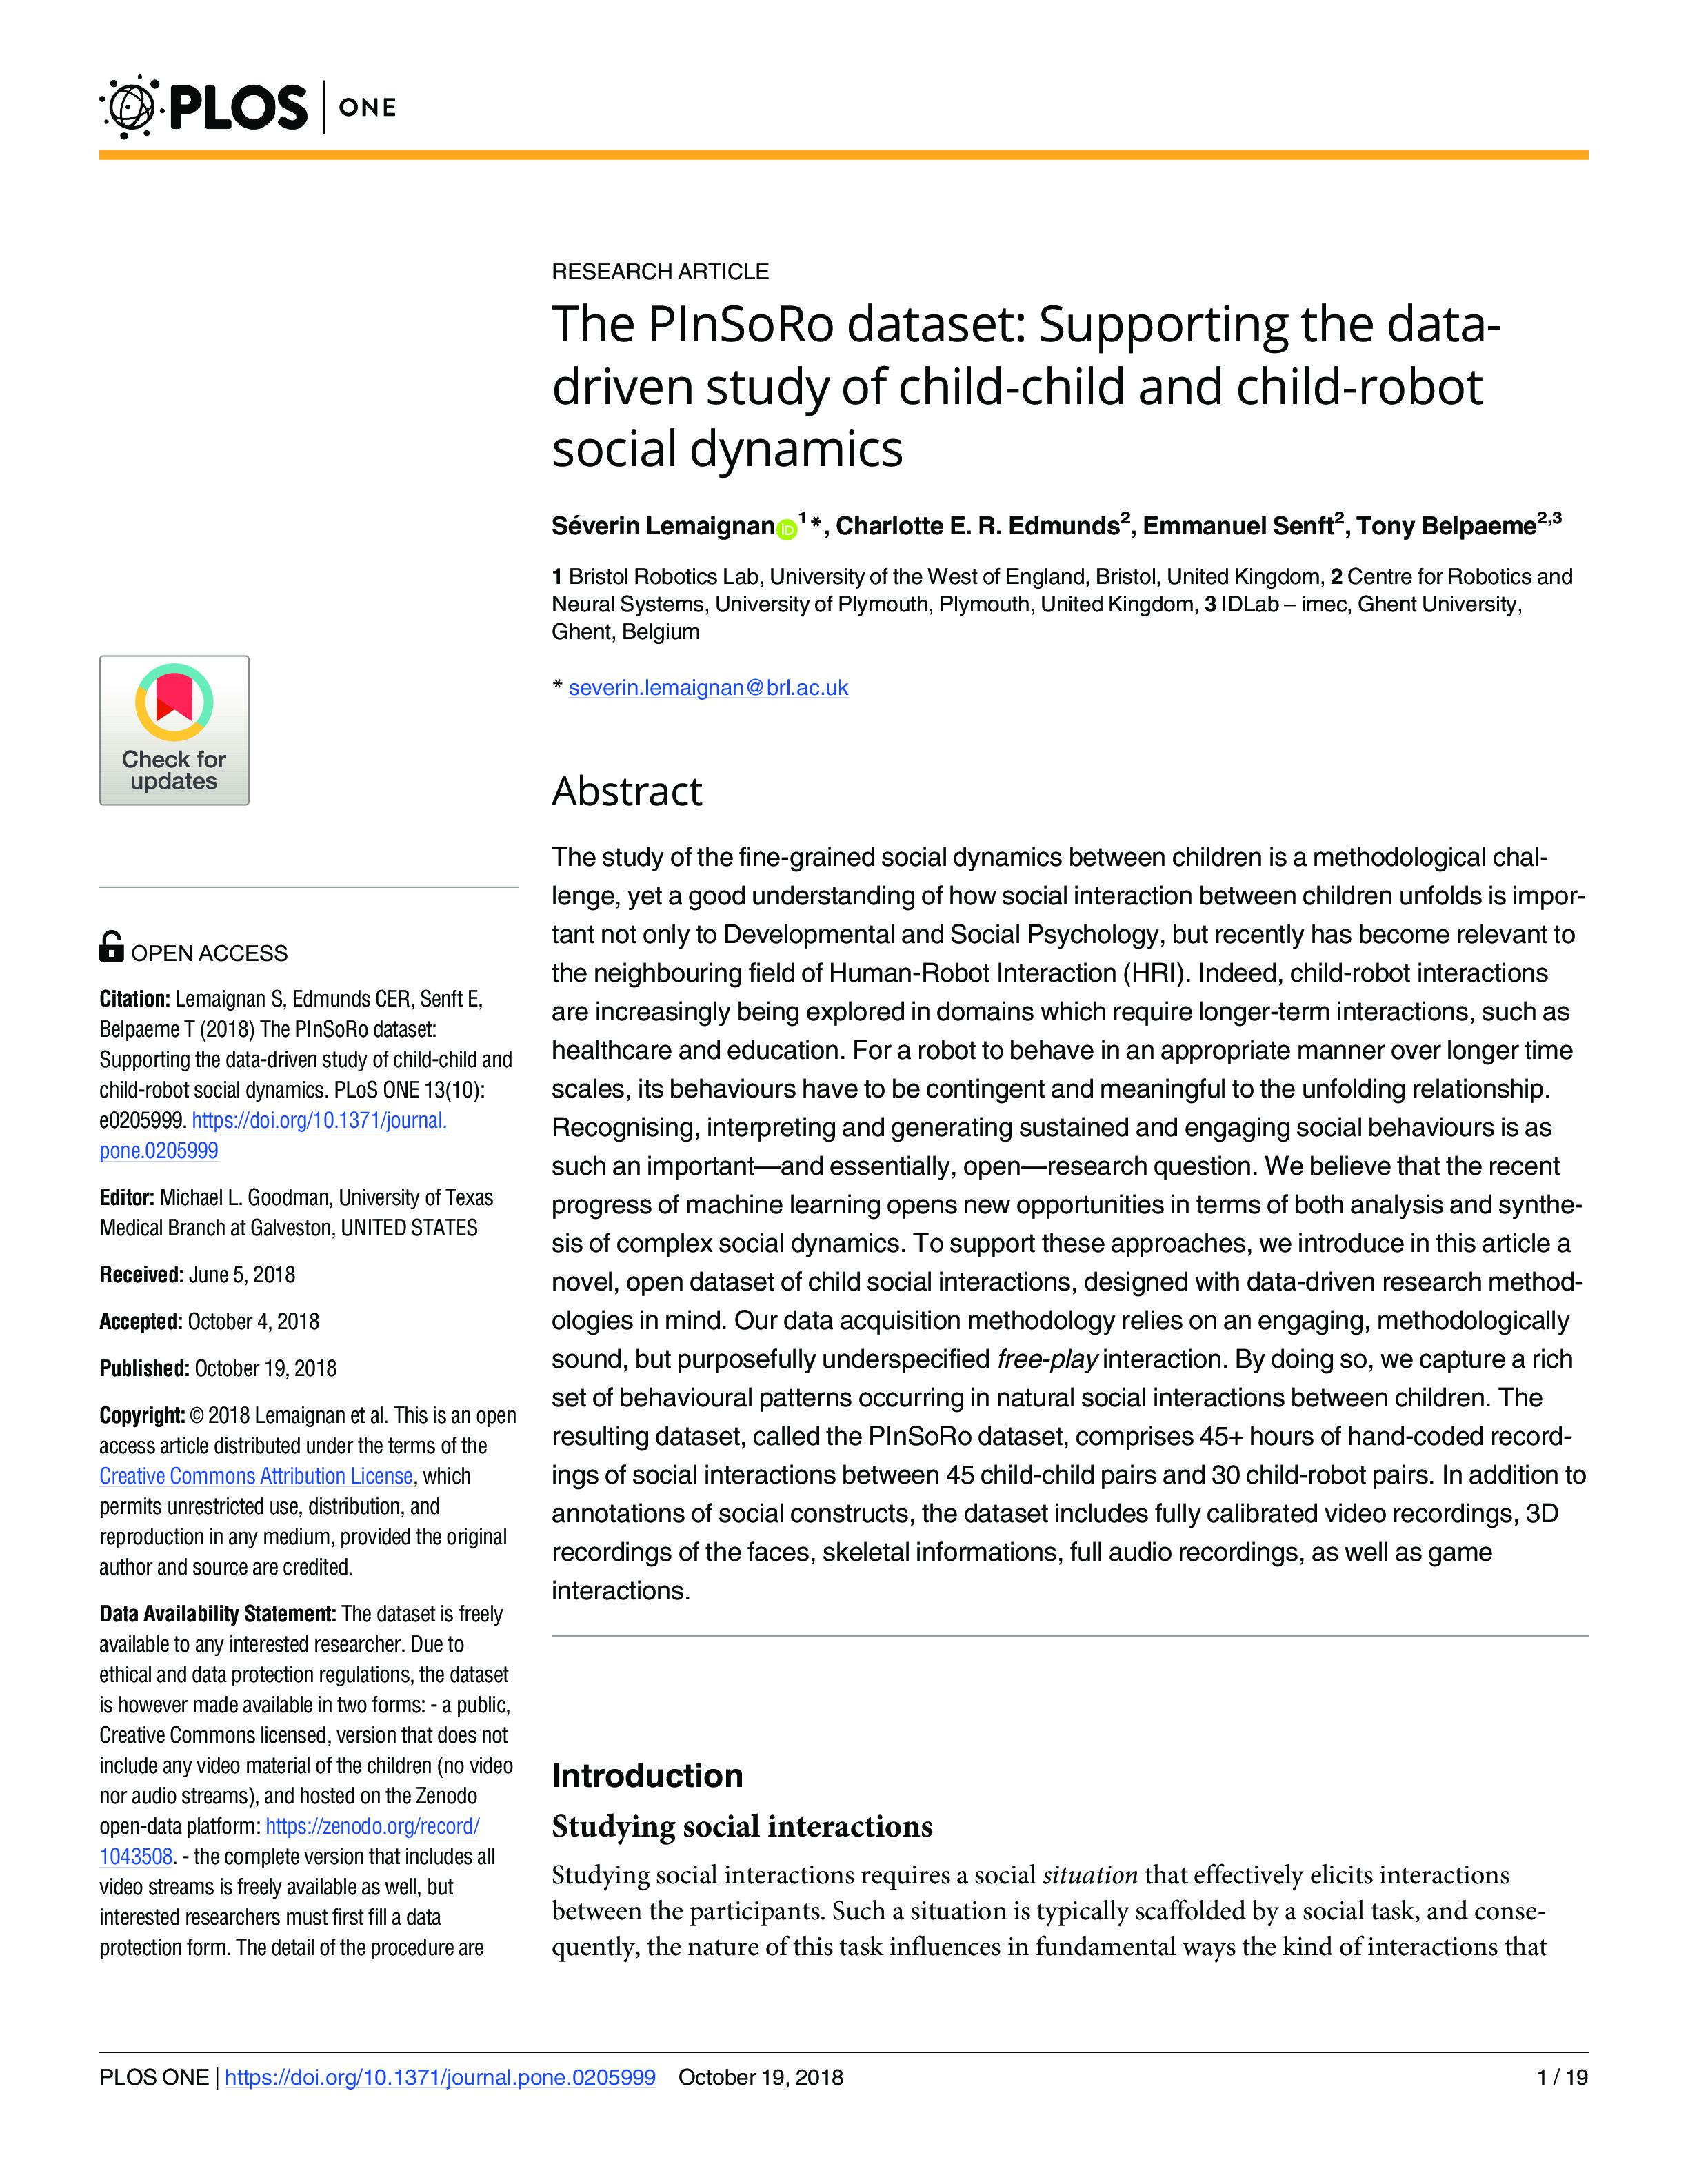
\includegraphics[height=2.2cm]{thumbs/2018-plosone.jpg} &

    \ul{Lemaignan, S.}, Edmunds E. R., C., Senft, E., Belpaeme, T.
    \newline\href{https://doi.org/10.1371/journal.pone.0205999}{\textbf{The
    PInSoRo dataset: Supporting the data-driven study of child-robot social
    dynamics}}
    \newline \textit{PLOS ONE} 2018
    & \small A first-in-kind, large scale dataset of child-child and child-robot social interactions. Design
    with machine learning in mind, this dataset effectively opens up the field
    of data-driven social psychology, with direct applications in AI and social
    robotics.\textbf{[principal investigator]}\\

    \vspace{-.20cm}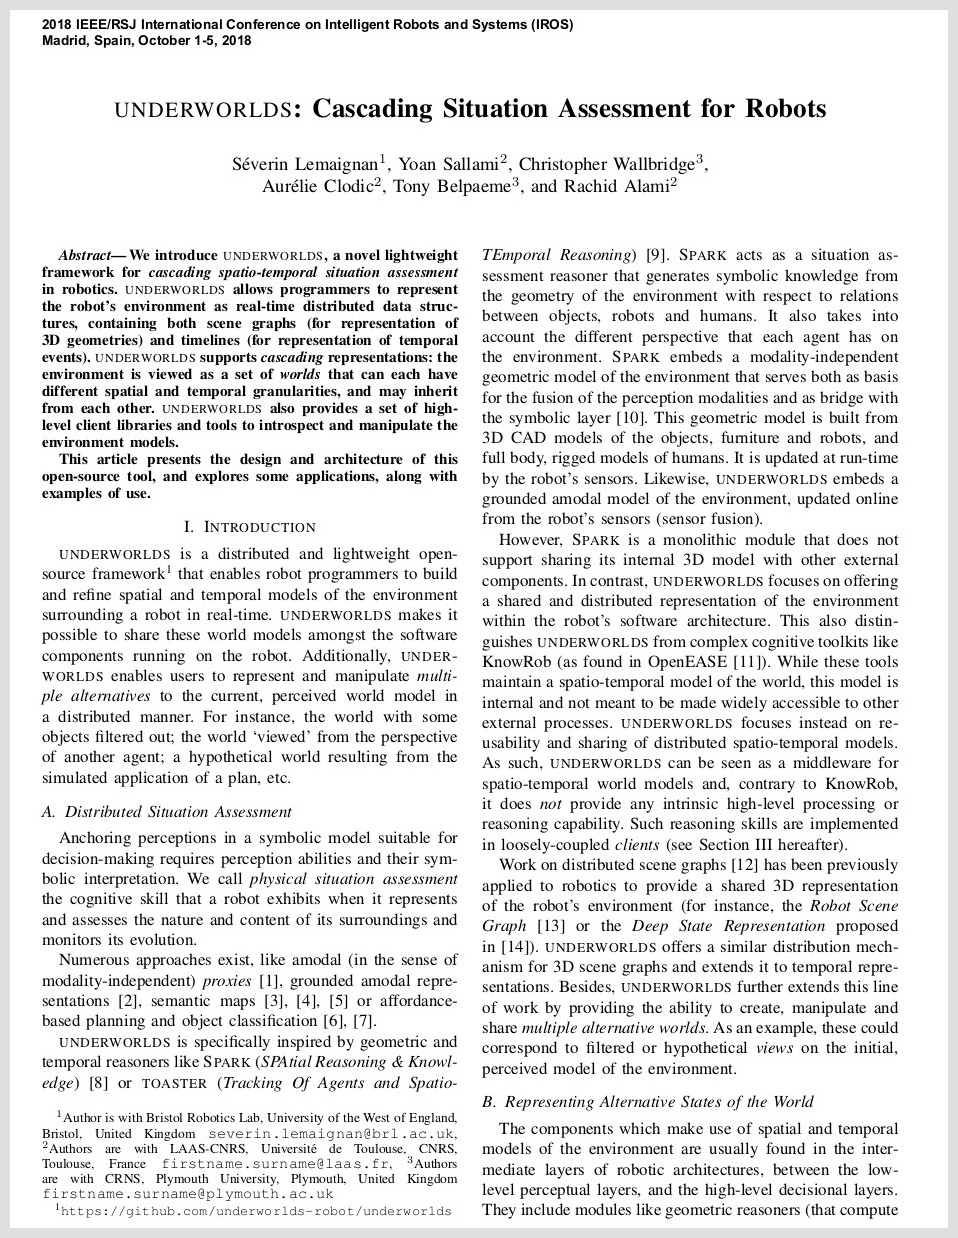
\includegraphics[height=2.2cm]{thumbs/2018-underworlds.jpg} &

    \ul{Lemaignan, S.}, Sallami, Y., Wallbridge, C., Clodic, A., Alami,
    R. 
   \newline\href{https://doi.org/10.1109/IROS.2018.8594094}{\textbf{\sc
    underworlds: Cascading Situation Assessment for Robots}}
    \newline\textit{IEEE IROS} 2018

    & \small A novel representation technique to efficiently
    represent multiple parallel states of the world, including imaginary ones.
    This ability is critical to represent spatio-temporal predictions, and to
    create models of other agents' representations.
    \textbf{[principal investigator]}\\



    \vspace{-.20cm}
\includegraphics[height=2.2cm]{thumbs/2017-sparc.jpg} &

    Senft, E., Baxter, P., Kennedy, J., \ul{Lemaignan, S.}, Belpaeme, T.
    \newline\href{https://doi.org/10.1016/j.patrec.2017.03.015}{\textbf{Supervised
    Autonomy for Online Learning in Human-Robot Interaction}}
    \newline \textit{Pattern Recognition Letters} 2017
    & \small The mathematical and technical bases of the SPARC
    paradigm for human-in-the-loop machine learning, showing that
    high-dimensional problems can be learnt effectively and rapidely thanks to
    an innovative input feature selection mechanism.
    \textbf{\newline[student supervisor; 22 citations]}\\


    \vspace{-.20cm}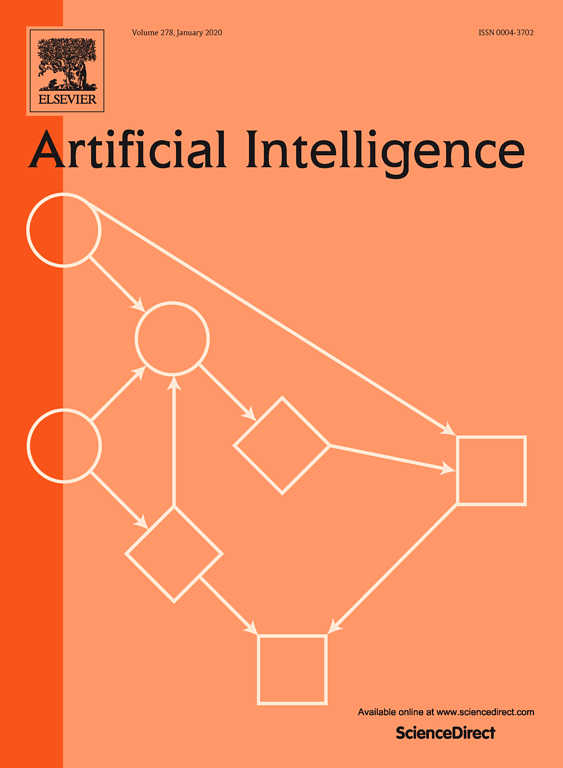
\includegraphics[height=2.2cm]{thumbs/2017-ai-cover.jpg} &

    \ul{Lemaignan, S.}, Warnier, M., Sisbot, E.A., Clodic, A., Alami, R.
    \newline
    \href{https://doi.org/10.1016/j.artint.2016.07.002}{\textbf{Artificial
    Cognition for Social Human-Robot Interaction: An Implementation}}
    \newline \textit{Artificial Intelligence} 2017
    & \small Landmark article: one of the first complete, semantic-aware, robotic architecture for
    human-robot interaction, including symbolic knowledge representation,
    situation assessment, natural language grounding, task planning, human-aware
    motion planning and execution. \textbf{\newline[principal investigator and
    coordinator; 140 citations]}\\


    \vspace{-.20cm}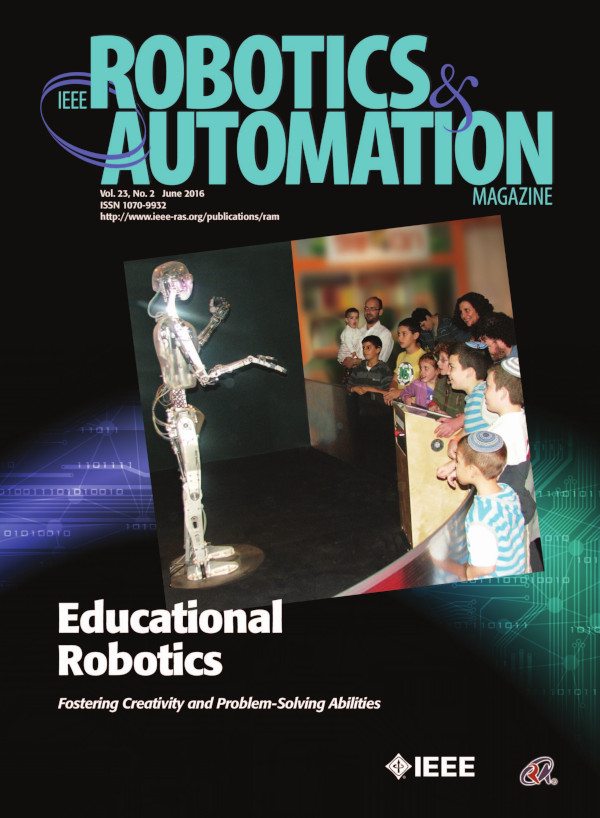
\includegraphics[height=2.2cm]{thumbs/2016-cowriter.jpg} &

    \ul{Lemaignan, S.}, Jacq, A., Hood, D., Garcia, F., Paiva, A., Dillenbourg, P.
    \newline
    \href{https://doi.org/10.1109/MRA.2016.2546700}{\textbf{Learning by
    Teaching a Robot: The Case of Handwriting}}
    \newline \textit{Robotics and Automation Magazine} 2016
    & \small Long-term studies with children and
    therapists, where we \emph{reverse} the social role of the
    robot to significantly improve the children' self-confidence. A landmark in
    social robotics for education. \textbf{\newline[principal investigator; 141
    citations} (incl. conf. article) \textbf{]}\\


    \vspace{-.20cm}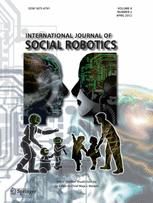
\includegraphics[height=2.2cm]{thumbs/2012-grounding.jpg} &

    \ul{Lemaignan, S.}, Ros, R., Sisbot, E. A., Alami, R., Beetz M.
    \href{https://doi.org/10.1007/s12369-011-0123-x}{\textbf{Grounding
    the Interaction: Anchoring Situated Discourse in Everyday Human-Robot
    Interaction}} 
    \newline \textit{Intl Journal of Social Robotics} 2012

    & \small In this paper, I show how symbolic knowledge representation can be
    used by robot to ground natural language interactions, also taking into
    account the unique perspective of the human interactor.
    \textbf{\newline[principal investigator; 100 citations]}\\

    \vspace{-.20cm}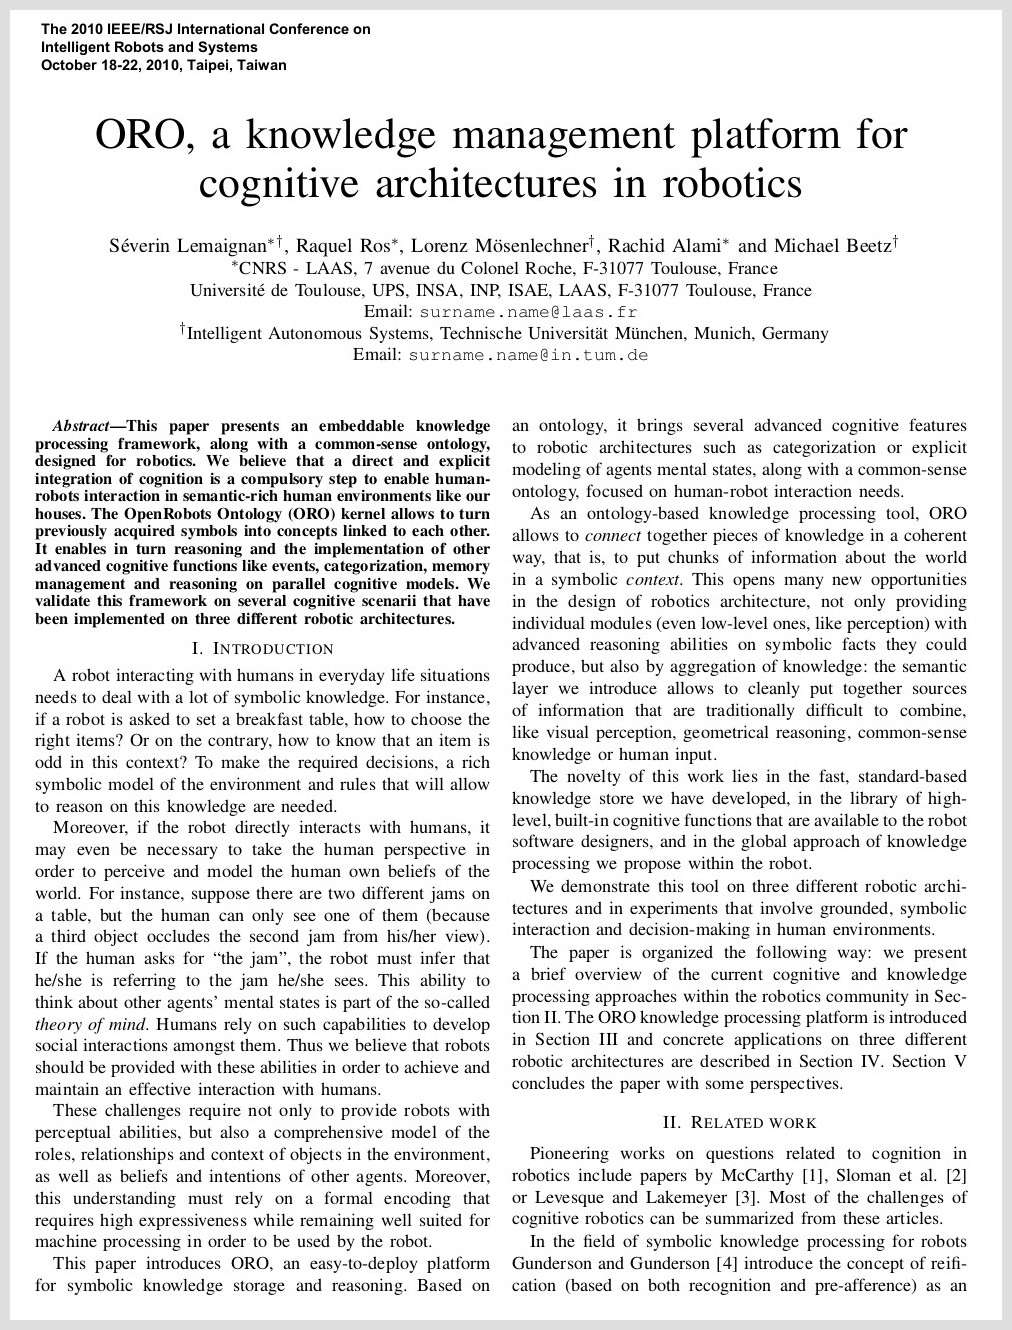
\includegraphics[height=2.2cm]{thumbs/2010-oro.jpg} &
    \ul{Lemaignan, S.}, Ros, R., Mösenlechner, L., Alami, R., Beetz, M.
    \newline\href{https://doi.org/10.1109/IROS.2010.5649547}{\textbf{ORO, a Knowledge Management Module for Cognitive Architectures in
    Robotics}}
    \newline \textit{IEEE IROS} 2010

    & \small One of the very first knowledge base designed and
    integrated in service robots. Pioneering work which played a key role in
    understanding how intelligent robot can represent their
    knowledge to facilitate communication with humans.
    \textbf{\newline[principal investigator; 155 citations]}\\

\end{tabular}
%}



\subsection{Peer recognition}

\begin{tabular}{p{0.15\linewidth}p{0.8\linewidth}}
    \bf 2023 & {\bf chosen as General Chair of the HRI'25 conference} \\
    \bf 2020 & {\bf invited to the international HRI Steering Committee} \\
    \bf 2015 -- 2017 & {\bf EU Marie Skłodowska-Curie Individual Fellowship}
    Theory of Mind and social robotics    \newline Plymouth University, UK \\
    \bf HRI'2017  & Best Paper award\\
    \bf HRI'2016  & Best Paper award\\
    \bf 2012         & {\bf Best PhD in Robotics 2012} award, CNRS, France \\
\end{tabular}

\section{Additional Information}

\subsection{Career breaks, diverse career paths and major life events}

\eu{You may include a short factual explanation of career breaks or diverse career paths such as secondments, volunteering, part-time work, time spent in different sectors or the effects of major life events such as long term illness as well as the effects of pandemic restrictions on research productivity.}

\subsection{Other contributions to the research community}

\eu{You may include a list of particularly noteworthy contributions to the research community you have made other than research achievements and peer recognition and a short explanation of these contributions. The purpose of this section is to allow the panels to take a more rounded view of your career and achievements and to ensure that any additional responsibilities, commitments and leadership roles that you have taken on beyond your individual research activities are recognised and taken into account.}

%%%%%%%%%%%%%%%%%%%%%%%%%%%%%%%%%%%%%%%%%%%%%%%%%%%%%%%%%%%%%%%%%%%%%%%%%%%%%
%%%%%%%%%%%%%%%%%%%%%%%%%%%%%%%%%%%%%%%%%%%%%%%%%%%%%%%%%%%%%%%%%%%%%%%%%%%%%
%%%%%%%%%%%%%%%%%%%%%%%%%%%%%%%%%%%%%%%%%%%%%%%%%%%%%%%%%%%%%%%%%%%%%%%%%%%%%

%I \textbf{contributed significantly to the framing
%of the emerging field of data-driven HRI}, also releasing of the PInSoRo open
%dataset (\href{https://doi.org/10.5281/zenodo.1043507}{10.5281/zenodo.1043507}),
%a \textbf{one-in-a-kind dataset of child-child and child-robot social
%interactions}.
%


%\subsection{Host institution}\label{host-institution}}
%
%The \emph{Bristol Robotics Laboratory (BRL)} is the largest co-located
%and most comprehensive advanced robotics research establishment in the
%UK. It is a joint venture between the University of the West of England
%and the University of Bristol. BRL's multidisciplinary approach aims to
%create autonomous devices capable of working independently, with each
%other, or with humans. BRL draws on robotics, electrical \& mechanical
%engineering, computer science, psychology, cognitive science and
%sociology. BRL has an international reputation as a leading research
%centre in advanced robotics research and has over 250 researchers
%working on a broad portfolio of topics: HRI, collective robotics, aerial
%robotics, neuro-inspired control, haptics, control systems, energy
%harvesting and self-sustaining systems, rehabilitation robotics, soft
%robotics and biomedical systems. BRL has many collaboration
%partnerships, both national and international, and is experienced in
%managing large multi-site projects. BRL has support from two embedded
%units specialising in business and enterprise, together with an
%incubator and successful track record of spin-outs.







%%%%%%%%%%%%%%%%%%%%%%%%%%%%%%%%%%%%%%%%%%%%%%%%%%%%%%%%%%%%%%%%%%%%%%%%%%%%%
%%%%%%%%%%%%%%%%%%%%%%%%%%%%%%%%%%%%%%%%%%%%%%%%%%%%%%%%%%%%%%%%%%%%%%%%%%%%%
%%%%%%%%%%%%%%%%%%%%%%%%%%%%%%%%%%%%%%%%%%%%%%%%%%%%%%%%%%%%%%%%%%%%%%%%%%%%%
%\newpage

\fancyhead[L]{Lemaignan, \project{}, Part B2}


\TODO{TOTAL BUDGET: 14 pages}

\TODO{TENTATIVE TARGET PAGE BUDGET: 4 pages: state of art + vision; 2 pages: methodology overview; 5 pages:
WPs; 3 pages: ethics + risks}

\tableofcontents

\newpage

\newrefsection
\chapter{B2.a State-of-the-art and objectives}

\eu{(B2.a, B2.b: max 14 pages}
\eu{

Section a: State-of-the-art and objectives. Specify the proposal objectives in
the context of the state of the art in the research field. It should be clear
how and why the proposed work is important for the field, and what impact it
will have if successful, such as how it may open up new horizons or
opportunities for science, technology or scholarship. Specify any particularly
challenging or unconventional aspects of the proposal, including multi- or
inter-disciplinary aspects.


Section B: Methodology. Describe the proposed methodology in detail including
any key intermediate goals. Explain and justify the methodology in relation to
the state of the art. Highlight any intermediate stages where results may
require adjustments to the project planning. In case you ask that team members
are engaged by another host institution, their participation has to be fully
justified by the scientific added value they bring to the project.  }

%%%%%%%%%%%%%%%%%%%%%%%%%%%%%%%%%%%%%%%%%%%%%%%%%%%%%%%%%%%%%%%%%%%%%%%%%%%
%%%%%%%%%%%%%%%%%%%%%%%%%%%%%%%%%%%%%%%%%%%%%%%%%%%%%%%%%%%%%%%%%%%%%%%%%%%
%%%%%%%%%%%%%%%%%%%%%%%%%%%%%%%%%%%%%%%%%%%%%%%%%%%%%%%%%%%%%%%%%%%%%%%%%%%
\section{A. State-of-art and objectives}

\subsection{PartB1 intro}
Social situations -- i.e. \emph{temporally and spatially bounded series of
events abstracted by the observer from the on-going flow of social life}, as put
by Garbett in~\cite{garbett1970analysis} -- are a fundamental building block in
social psychology~\cite{argyle1981social}. When specifically looking at
artificial agents like social robots, making sense of these situations is
critical: their level of social cognition depends on their ability to identify,
interpret and interact with the world surrounding
them~\cite{szczepanowski2017computational}, and in particular, correctly
interpret transactions of social signals -- specific events in which an agent
performs a social action aimed at another agent~\cite{pantic2011social}. This
socio-cognitive skill, \emph{social situation awareness}, is essential to build
intelligent social agents.

\TODO{rephrase -> Endsley situation awareness is not exactly the same thing}

Endsley identifies in~\cite{endsley1995theory} three levels to the related concept
of \textit{situation awareness} (SA) :\emph{perception}, \emph{comprehension}, and
\emph{projection of future states}. Applied to social situation awareness,
the \emph{perception} of social signals has already been studied in depth in the
community~\cite{pantic2011social,vinciarelli2009social}.  However, relating the
resulting percepts into a comprehensive representation of a social situation
(\emph{comprehension}) and reasoning about this representation to derive an
interpretation (for instance, in terms of \emph{projections} of future social
states) are hard problems that arguably hinder further progress in social AI and
robotics~\cite{yang2018grand}. Current research is fragmented, and proposed
methods are either abstract models~\cite{gordon2016commonsense}, or task-specfic
approaches: for instance, group activity
recognition~\cite{shu2017cern,wu2019learning}; pedestrians modelling for robotic
social navigation~\cite{alahi2016social}; on-going state of an
interaction~\cite{garcía2020explainable}. We are however lacking a more
principled, general methodology to represent and reason about complex social
situations. As put by Scassellati in 2018 in the \emph{Science Robotics}' list of
ten Grand Challenges for Robotics~\cite{yang2018grand}, \emph{we have very few
comprehensive, quantitative analyses of human social responses}, and little
progress has been achieved since then.

\project aims at a breakthrough on that issue, and introduces the fundamentally new
idea of \emph{social embeddings}: a data-driven and semantics-preserving
computational representation of contextualized social situations.  As presented
below, social embeddings represent a paradigm shift for the domain: they open
the way to generic, task-agnostic representations and quantitative measurement
of the social situations in which an agent is embedded, something that was until
now only possible using time-consuming qualitative methodologies or
non-generalizable model-based techniques.  The results of \project have the
potential to significantly accelerate the development of generic artifical
agents that are socially-aware, also creating an interdiscplinary bridge between
the current trends in machine learning, social robotics, and a broad range of discipline relying
on data-driven social sciences.



%%%%%%%%%%%%%%%%%%%%%%%%%%%%%%%%%%%%%%%%%%%%%%%%%%%%%%%%%%%%%%%%%%%%%%%%%%%
\subsection{State-of-art: social representations for intelligent robots}

Correctly interpreting our social environment is complex for machines, and has
long been identified as a key challenge on the road to competent social
robots~\cite{yang2018grand}. Accordingly, a significant, and growing, amount of
research has been dedicated to this question over the past 15
years~\cite{bartneck2020human}, without however satisfactorily coming to a
conclusion.

Let's consider the following simple illustrative example: a waiter, serving
customer in a restaurant, tell a joke. The guests look at him, smile and laugh,
and go on with ordering their dinner. As social beings, we can easily interpret
this simple description, and understand that the waiter is friendly, the guest
in a good mood, and the overall interaction is going well. Let's now consider
the same example, but the patrons do not laugh. This indicates that either the
joke was not appropriate in this context, or that the guests are not in the mood
for a joke. Either way, the interaction is not satisfactory. Finally, let
consider the same example, but this time, the waiter did not tell any joke and
was simply taking orders. Still, the guests start laughing. In this context, the
unexpected laughing tells us that something went wrong with the waiter's
behaviour.  Laughing is a relatively simple social signal to detect for a robot,
but without proper representation of the social and physical context -- and its
attached social norms -- a robot-waiter would not be able to properly understand
the situation.

To effectively interpret this situation, a robot needs a \emph{joint}
computational model of (1) the social agents relevant to the situation; (2) the
physical environment (locations and relationships between objects and other
spatial features); (3) the plans, on-going actions, and predicted results of the
tasks performed both by the robot and by the other agents; (4) a common-sense
knowledge of the social rules and norms associated to this task and context.

In addition, models for (1), (2) and (3) also have to represent \emph{dynamics} as
well: changes in the agents' behaviours, expressions, interactions; expected or
unexpected changes in the physical environment; change of plans and actions.

We review below the main approaches to build models for each of these four
aspects, as well as existing attempts to build complete models of social situations.


\subsubsection{Modelling social agents and social groups}



The importance of correctly interpreting non-verbal cues, such as facial
expressions, body language, and prosody, along with the verbal content, is well
understood in robotics as required to comprehend the emotional state and
intentions of the humans it interacts with~\cite{breazeal2003emotion}.

While the \emph{perception} of social signal has been studied in depth in the
HRI community (for instance,~\cite{pantic2011social}), and the \emph{evaluation} of
the social situation is usually handled as an aspect of the robot's decision
making, the \emph{interpretation} of social situations is a difficult problem.
It requires to build and maintain a task-appropriate model of the situations,
and represent it in such a way that a machine can reason about it.


\subsubsection{Modelling the physical context}

\subsubsection{Task modelling and action prediction}



Moreover, in a service context like a restaurant, where a robot may take on a
role similar to a waiter, misreading a social cue can lead to a breakdown in
service quality or even disrupt the customer experience. For instance, failing
to recognize a patron's displeasure with a joke might lead to repeated behavior
that further damages the relationship, whereas a socially aware robot could
adapt its interaction strategy, perhaps by offering an apology and altering its
behavior to better align with the guests' preferences~\cite{mutlu2006storytelling}.

\subsubsection{Modelling social norms}

Therefore, developing a concise representation of social situations for
autonomous social robots is crucial. Such a representation should include the
ability to model and predict the outcomes of social interactions, incorporating
an understanding of social norms, cultural context, and the potential
ramifications of deviating from expected behaviors. By doing so, social robots
can achieve a more natural and effective integration into human social spaces,
fostering positive human-robot interactions and ensuring the success of their
service functions~\cite{gockley2005designing}.


\subsubsection{Joint models of social situations}



Artificial social intelligence~\cite{bainbridge1994artificial}

researchers describe the results of social
interaction as a function not only of the individuals involved
but also of the social situation~\cite{rusbult2003interdependence}

Sociologists and social psychologists have long
recognized the importance of the situation as a determining
factor of interpersonal interaction: Atlas of Interpersonal Situations~\cite{kelley2003atlas}

Social psychologists, on the other hand, have long
considered the situation-specific aspects of interpersonal
interaction [9]. The use of social situations for examining
social interaction is widespread within both neuroscience [16]
and experimental economics [17]. Interdependence theory is a
social psychological theory developed as a means for
understanding and analyzing interpersonal situations and
interaction [9]. The term interdependence describes the extent
to which one individual of a dyad influences the other.

Wagner's \emph{outcome matrices}
\cite{wagner2006framework} \cite{wagner2009creating}

Mutual modelling:
\cite{dillenbourg2016symmetry}
stereotyping: \cite{wagner2015robots}


\TODO{copy paste from part b1}

Endsley identify in~\cite{endsley1995theory} three levels to the related concept
of \textit{situational awareness} :\emph{perception}, \emph{comprehension}, and
\emph{projection of future states}. Applied to social situation awareness,
the \emph{perception} of social signals has already been studied in depth in the
community~\cite{pantic2011social,vinciarelli2009social}.  However, relating the
resulting percepts into a comprehensive representation of a social situation
(\emph{comprehension}) and reasoning about this representation to derive an
interpretation (for instance, in terms of \emph{projections} of future social
states) are hard problems that arguably hinder further progress in social AI and
robotics~\cite{yang2018grand}. Current research is fragmented, and proposed
methods are either abstract models~\cite{gordon2016commonsense}, or task-specfic
approaches: for instance, group activity
recognition~\cite{shu2017cern,wu2019learning}; pedestrians modelling for robotic
social navigation~\cite{alahi2016social}; on-going state of an
interaction~\cite{garcía2020explainable}. We are however lacking a more
principled, general methodology to represent and reason about complex social
situations. As put by Scassellati in 2018 in the \emph{Science Robotics}' list of
ten Grand Challenges for Robotics~\cite{yang2018grand}, \emph{we have very few
comprehensive, quantitative analyses of human social responses}, and little
progress has been achieved since then.


\subsubsection{The gap in our knowledge: holistic social situations
representations}


\subsection{Embeddings as representations for social situations}

\subsubsection{Embeddings in Machine Learning}

In the context of machine learning, we refer to an \emph{embedding} as a
real-valued vector representation of a typically much higher dimensionality
input. In other words, a representation that encodes high-dimensionality input
(for instance, an image) into a lower-dimensional space. Critically, embeddings
are trained to encode the relationships and semantic nuances that might exist in
the original input space. For instance, two pictures of the same face
transformed with an embedding tuned for facial recognition would yield two
vectors that are similar to each other (i.e., close to each other for a given
metric, usually the cosine distance). As such, the process of embedding not only
condenses high-dimensional information into a more manageable form but also
captures latent associations that might otherwise remain
obscured~\cite{bengio2009learning}.

Unsurprisingly, the training of compact yet semantically-rich embeddings has
been a very active research topic over the last two decades, yielding
exceptional results in machine learning, where the (otherwise high)
dimensionality of real-world percepts might turn common machine learning
tasks like classification or prediction intractable.

While research on embeddings initially focused on data that would intuitively
lend itself well to mathematical transformations (for instance, reducing the
dimensionality of an image, represented as an array of pixel intensities, or
processing sound), it has since then been discovered that many constructs --
physical or not -- can also be \emph{embedded} in a low-dimension numerical
space, while preserving many of their semantics. One of the landmark
achievements in that regard is the work published in 2013 by Mikolov et al. --
themselves building on previous work spanning another decade.  They showed that
embeddings can be computed for \emph{words}, also encoding some of their
semantic meaning~\cite{mikolov2013efficient}, with the famous example of
\emph{embedding(`king') - embedding(`man') + embedding(`woman') $\approx$
embedding(`queen')}. Effectively, a conceptual equivalence of terms, involving
semantics related to gender and social role could be transformed into simple
mathematical additions and subtractions.

This outcome ushered in a decade of intense research on text representation,
ultimately resulting in the current Large Language Models (LLM) like GPT or
Llama2.  Most of the recent progress has been enabled by the discovery in 2017
of the attention-based \emph{Transformers}~\cite{vaswani2017attention} neural
network structure, which brought a boost to the research on natural language
procesing with, for instance, BERT~\cite{devlin2019bert} in 2019 and the family
of GPT models~\cite{wolf2020transformers} in 2020.  These large models
are pre-trained on massive text corpora and are typically used for token
prediction (the pre-trained network is fed with a text context, and predicts the
next tokens).  Importantly for this work, these very large pre-trained networks
can also be used to compute text-level embeddings, representing a short text as
a numerical vector~\cite{reimers2019sentencebert,muennighoff2022sgpt}. The
resulting embeddings can be then used to measure text-relatedness for instance,
as in the BEIR benchmark~\cite{thakur2021beir}.

\subsubsection{Social embeddings}

\begin{rewrite}
Combining the above concepts of social situations and text embeddings, we introduce in
this paper the idea of \emph{social embeddings}. A \emph{social embedding} is a
compact, real-valued numerical representation (a vector) of a social
situation, as experienced by an agent immersed in that social environment.
Following the general idea of embeddings, social embeddings are designed
to encode the \emph{semantics} of the social situation currently experienced by
the agent, facilitating the interpretation of the situation. For instance, it
could make it straightforward to compare two social situation by simply
measuring how similar the two corresponding embeddings are.

The key insight to construct these embeddings is to exploit the social knowledge
already encoded in the latent space of large language models. We do so by
automatically generating a textual description of the social environment of the
robot (using regular perception routines), and by transforming this
description into a text embedding via a large language model. By doing so, we
effectively construct an \emph{embedding}, i.e., a projection, of the social
space into a machine-friendly numerical space.

This article is a first investigation of this idea. In the following sections,
we start the exploration of the design space of social embeddings by presenting
a simple algorithm to generate scene descriptions and derive embeddings; we
analyse and discuss several key characteristics and parameters of the derived
embeddings -- like their application as a quantitative \emph{social distance};
and we discuss several promising directions for follow-up research.

\end{rewrite}

%%%%%%%%%%%%%%%%%%%%%%%%%%%%%%%%%%%%%%%%%%%%%%%%%%%%%%%%%%%%%%%%%%%%%%%%%%%
\subsection{Objectives of \project}
\label{sec:objectives}

%\project is built around three axes: a basic research programme; an experimental
%programme that looks specifically at the application of social embeddings to
%social robotics; and, running in parallel to those first two axes, a scientific
%investigation of the ethical dimension of social embeddings.

This idea of \emph{social embeddings} builds on a proof-of-concept that I
validated in~\cite{lemaignan2024social}. \project will turn that early concept
into a mature mathematical tool for social sciences and artificial social
agents. As I explain below, I will formalize their construction,  fully
characterise their properties, expand their scope to complex, real-world social
situations, and demonstrate their transformative potential through deployment of
socially intelligent robots in multiple experimental settings.

\vspace{1em}

\noindent At the basic research level, \project targets two overarching research goals:

\begin{enumerate}[label=\textbf{(\arabic*)}]
    \item to build compact, yet semantics-preserving, embeddings to represent
arbitrary social situations; and to fully characterize these embeddings,
including their latent semantics. I translate this first goal into objective
{\bf O1}:

\begin{enumerate}[label=\textbf{O\arabic*}]
    \item \label{O1} To \textbf{construct and characterize the fundamental
properties of social embeddings}.
\end{enumerate}

    \item to precisely \textbf{define and implement the socio-cognitive skill of
        \emph{social sitation awareness} enabled by social embeddings}. I split this
        second goal into three specific objectives: \emph{social appraisal},
        \emph{social prediction}, \emph{social learning}.

\begin{enumerate}[label=\textbf{O2.\arabic*}]
    \item \label{O2.1} To use social embeddings to \textbf{automatically appraise
        social situations}, taking into account their \textbf{context}. Using
        a set of prototypical reference situations~\cite{kelley2003atlas}, social embeddings
        can be used to relate the current social situation to known ones.
        Besides, because social embeddings lend themselves to jointly encode
        social context by simply attaching context descriptions, the appraisal
        of the social situation can be made \emph{context-aware};

    \item \label{O2.2} To use social embeddings to model \textbf{social
        dynamics} by characterizing the trajectories of on-going social situations in the
        embedding space. I will look in particular into trajectories'
        \emph{discontinuties}, that might represent unexpected changes of social
        dynamics, and trajectories' \emph{extrapolations}, that might represent
        \textbf{social situation \emph{predictions}}.

    \item \label{O2.3} To \textbf{learn socially-appropriate behaviours} by using
        social embeddings as an additional input feature to existing robot behaviour
        generation algorithms, and by augmenting existing interactive machine
        learning techniques (`user in-the-loop' social learning for robots, that I
        pioneered in e.g.~\cite{winkle2021leador}) with
        representations of the social situation;

\end{enumerate}
\end{enumerate}

\noindent To illustrate these objectives, let consider the following imaginary
scenario: a robot is welcoming visitors at the entrance of an hospital; a group
of 3 persons are discussing together; one person is standing in the middle of
the room, glancing around; one last person is entering the hospital and
walks toward the reception. \ref{O2.1} will show that social embeddings can
represent and appraise this situation, accounting for the `hospital entrance' context: while
the person walking towards the reception probably does not need help from the
robot, the one in the middle seems uncertain, and might appreciate a pro-active
helping behaviour from the robot. \ref{O2.2} adds the temporal dimension: if we
sample the scene at regular time steps, and build a sequence of social
embeddings, what trajectory do they follow in the embedding space? Is it
continuous? Is there any rapid changes? Can we extrapolate this trajectory to
predict where the situation is going? \ref{O2.3}, finally, looks at exploiting
social embeddings for socially-aware behaviour learning. In our scenario, a
member of the hospital staff would for instance teach the robot an
context-appropriate response, and the robot would be able to generalise it to
other, similar social situations.


I want to evidence these properties in both lab-based experiments and
real-world deployments on social robots. Accordingly, \project has two addtional
objectives:

\begin{enumerate}[label=\textbf{O\arabic*}]
    \setcounter{enumi}{2}
    \item \label{O3} To fully {\bf integrate social embeddings onto a
        socio-cognitive architecture for autonomous service robots} and,

    \item \label{O4} To conduct an {\bf ambitious experimental programme} --
        including social observations, and both lab-based studies and field
        studies -- to demonstrate the effectiveness of social embeddings in
        complex, real world conditions.  This means deploying the \project robot
        into existing complex social eco-systems.
\end{enumerate}


%Once completed, these four objectives will provide solid theoretical and
%empirical foundations to social embeddings.
%
%Each of these four objectives involve both basic and experimental research,
%presented in the next section.


\subsubsection{Basic research objectives}

\subsubsection{Empirical research objectives}


%%%%%%%%%%%%%%%%%%%%%%%%%%%%%%%%%%%%%%%%%%%%%%%%%%%%%%%%%%%%%%%%%%%%%%%%%%%
\subsection{Importance and impact of the project}

\begin{rewrite}

Academically, the \project project represents a timely combination of
very recent advances in supervised machine learning for social robot
behaviour with a creative and interdisciplinary approach to the design
and automation of social robot behaviour. 
We will publish \project results in interdisciplinary and high-profile
discipline-specific journals (eg. Science Robotics; Frontiers in AI and
Robotics; Transaction in Human-Robot Interaction) and conferences (eg. AAAI,
HRI, RSS).

The dataset of social behaviours and social signals we will create and
distribute represents a one-in-a-kind resource for the human robot
interaction community, and the human data collection will be
transferable to research in other domains such as human-computer
interaction.

As \project will be deployed in a living lab environment, there is
significant scope for public outreach/engagement and media coverage,
which we will work with the BRL's media manager to maximise.


\project aims at building unique European capacity to assert leadership in this
domain, and, beyond the specific deliverables of this 5-years project,
establishing the PI as a world-leader in goal-driven, socially-responsible
robotics.

\end{rewrite}

%%%%%%%%%%%%%%%%%%%%%%%%%%%%%%%%%%%%%%%%%%%%%%%%%%%%%%%%%%%%%%%%%%%%%%%%%%%
\subsection{Interdiscplinary nature of the project}

My project aims at introducing a completely new approach to the represention of
social situations. While \project focuses on embodied artificial social agents
like social robots, the basic research that I will conduct (WP1 and WP2) is
essentially independent of the domain of application, and might impact the whole
subfield of digital humanities related to the study of our social world.

Accordingly, the project is grounded in both the psycho-social literature of
human cognition, and the latest technological advances in artificial cognition
and human-robot interaction, and aims at delivering major conceptual, technical
and experimental contributions across several fields: intelligent robotics,
machine learning and AI, data-driven social psychology and sociology, ethics. By
working at the crossroad of these discipline, \textbf{\project builds bridges
across multiple disciplinary boundaries}.

\project delivers this programme using a range of scientific methods,
previously outlined in Part B1, combining for instance machine learning and
embedding-based data representation, with non-verbal social perception and field
observations of social behaviours.

Accordingly, the project builds on a \textbf{strong interdisciplinary team}: the
post-docs directly recruited on \project will have backgrounds in deep machine
learning (PD1) data-driven sociology (PD2, PHD1), cognitive modeling (PD3),
cognitive robotics (PHD2). Additional expertise will be recruited to provide
specific support: Dr. Maribel Pino and the Broca hospital living lab will
contribute their expertise on robot deployment and study orgnisation in an
hospital environment; the \project Ethics Advisory Board will contribute
expertise to guide the work on ethics.

%%%%%%%%%%%%%%%%%%%%%%%%%%%%%%%%%%%%%%%%%%%%%%%%%%%%%%%%%%%%%%%%%%%%%%%%%%%
%%%%%%%%%%%%%%%%%%%%%%%%%%%%%%%%%%%%%%%%%%%%%%%%%%%%%%%%%%%%%%%%%%%%%%%%%%%
%%%%%%%%%%%%%%%%%%%%%%%%%%%%%%%%%%%%%%%%%%%%%%%%%%%%%%%%%%%%%%%%%%%%%%%%%%%
\newpage
\section{B. Methodology}

%%%%%%%%%%%%%%%%%%%%%%%%%%%%%%%%%%%%%%%%%%%%%%%%%%%%%%%%%%%%%%%%%%%%%%%%%%%
\subsection{Overview of \project methodology}

\subsubsection{Research methodologies}

As presented in the Part B1, \project combines multiple scientific
methodologies to achieve the four objectives listed in
Section~\ref{sec:objectives}.



\subsubsection{Implementation of the work program}

I organise the project in four work-packages, aligned with the four objectives
(Figure~\ref{fig:wps}): \textbf{WP1} is dedicated to the construction and
characterization of social embeddings; \textbf{WP2} exploits social embeddings
to develop a new form of artifical social situation awareness; \textbf{WP3} looks at how
social robots can make use of this skill by integrating social embeddings into
existing cognitive architectures for service robots; and \textbf{WP4} organises
the experimental work, both lab-based and in-the-wild, that demonstrates the
\project approach in ambitious and complementary situations.


\begin{figure}[h!]
\centering
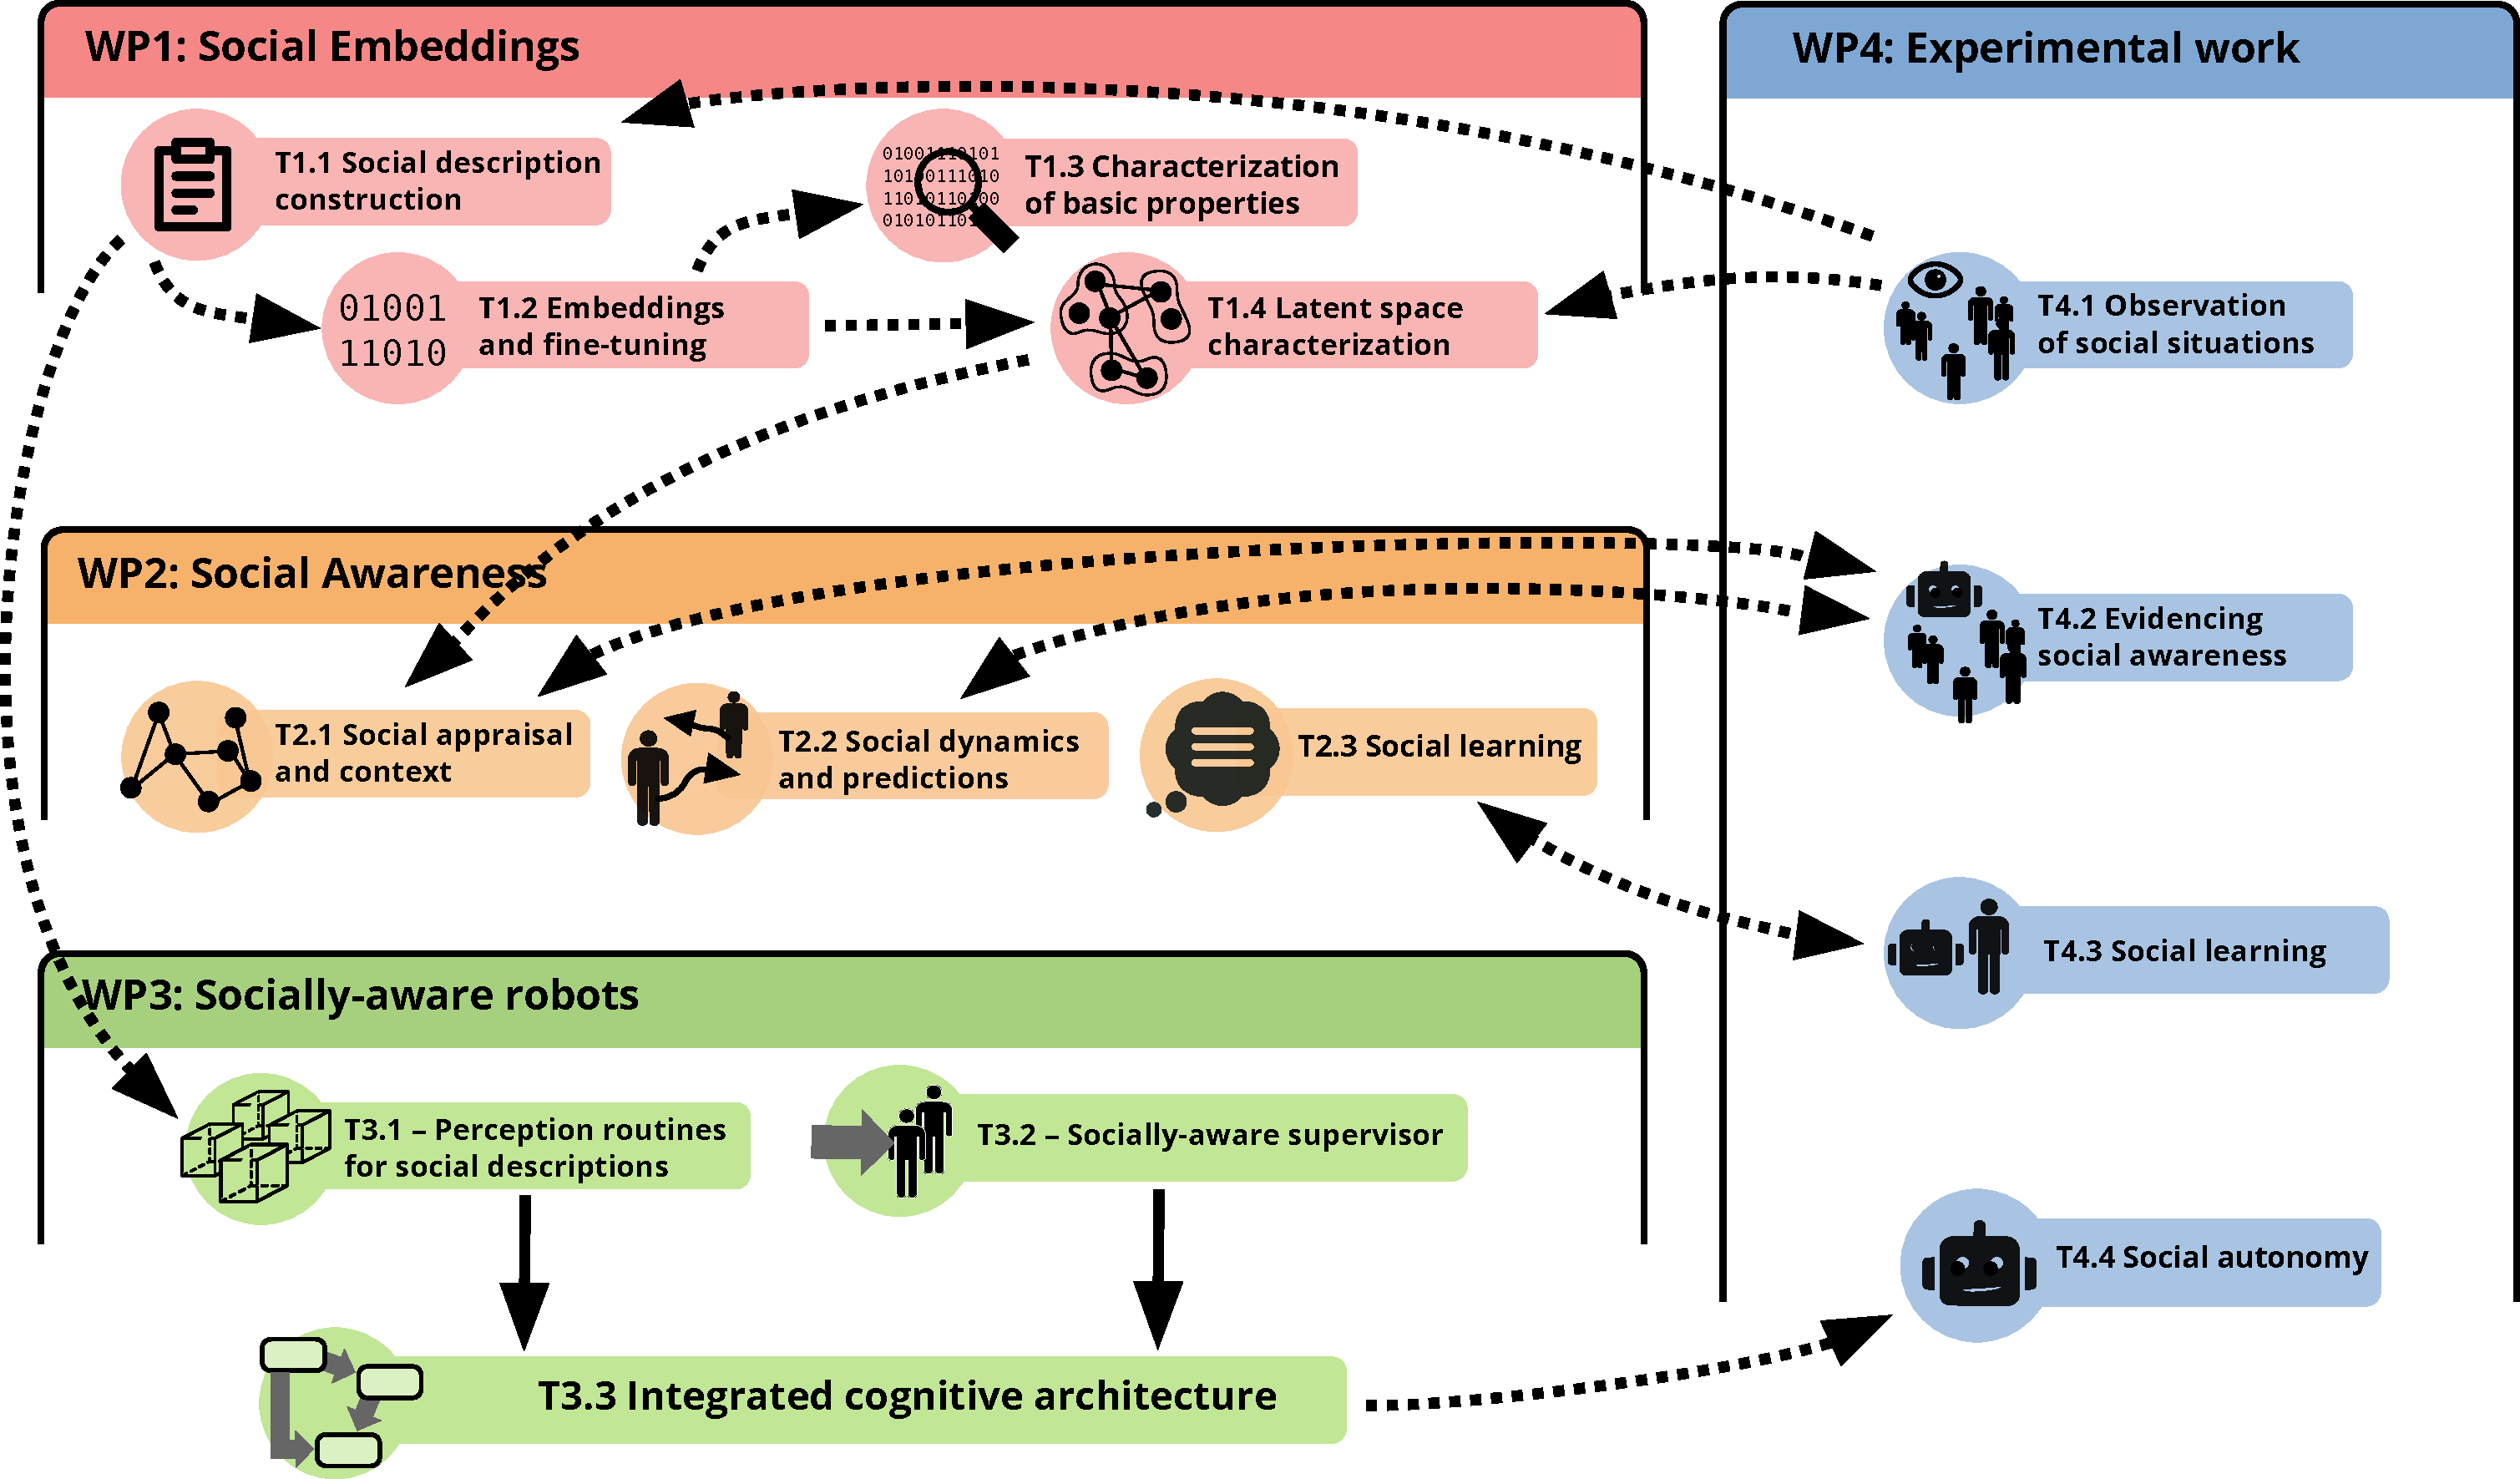
\includegraphics[height=0.6\linewidth]{figs/wps}
\caption{Overview of the workpackages and tasks, and tasks inter-relations.}
\label{fig:wps}
\end{figure}

More specifically, Figure~\ref{fig:wps} gives an overview of the project
workpackages, and their interrelations.


\subsubsection{Social Robotics as an experimental framework}

As a \emph{methodology} to represent and reason about social situations, social
embeddings are fundamentally agnostic from their final domain of application.
However, the practical study and validation of social embeddings does require
experimental grounding through artificial social agents embedded into
complex-enough social situations. In \project, I choose to exploit social robots
as an experimental platform.  Beyond my extensive experience and know-how in
social robotics, both at the basic level and at the experimental level, several
scientific and practical reasons drive this choice.

First, compared to many other AI systems (e.g. virtual avatars), robots
are physically situated.  They can partake to a broad range of naturalistic
social situations and social interactions, providing means to acquire,
fine-tune, and validate social embeddings in a variety of real-world scenarios.

Second, not only robots are physically situated, but they also have access to a rich
range of sensing modalities for social perception (including vision, audition).
Combined with robots' proprioception and localisation capabilities, these
percepts can be fully spatially-grounded. This let us compute a rich set of
social constructs (for instance, mutual gaze or joint attention), that feed
directly into the available social descriptors.

Third, social robots are \emph{active} social agents. From an experimental point
of view, robots' behaviours can be
designed to induce and influence specific social situations, providing us with a
invaluable tool to study social situations and related sociodynamics.

Finally, beyond the suitability of social robotics as an experimental
methodology for the \project project, the field of social robotics in itself is
``hitting a wall''~\cite{yang2018grand} in trying to build appropriate tools to represent and
reason about the social environment of robots. By specifically applying social
embeddings to social robotics, I also aim to provide new, groundbreaking
tools to the robotic community to build more intelligent social robots.

\subsubsection{Gantt chart}

%\begin{landscape}
%\begin{figure}[!h]
\resizebox{\linewidth}{!}{
    %%%%%%%%%%%%%%%%%
%%
%% Task dependencies
%%
%% Task...        depends on Task...
%% T1.3           T1.1
%% T1.3           T1.2
%% T1.2           T2.2 (user interface)
%% T3.3           T2.3
%%

\definecolor{barcolor}{RGB}{153,204,254}
\definecolor{linkred}{RGB}{165,0,33}
%\renewcommand\sfdefault{phv}
%\renewcommand\mddefault{mc}
%\renewcommand\bfdefault{bc}
\setganttlinklabel{s-s}{START-TO-START}
\setganttlinklabel{f-s}{}
\setganttlinklabel{f-f}{FINISH-TO-FINISH}

%\begin{sidewaysfigure}[!ht]
\begin{figure}[!ht]

%\sffamily
\begin{ganttchart}[
        canvas/.append style={fill=none, draw=black!5, line width=.75pt},
        hgrid style/.style={draw=black!5, line width=.75pt},
        vgrid={*1{draw=black!5, line width=.75pt}},
        %vgrid={*1{black}, *{11}{black!5}}, % doesnt work for some reason
        x unit=.35cm,
        y unit chart=.65cm,
        time slot format=isodate-yearmonth,
        time slot unit=month, % pgfgantt >= 5.0
        %compress calendar, % pgfgantt < 5.0 => overleaf
        title/.style={draw=none, fill=none},
        title label font=\bfseries\footnotesize,
        %title label node/.append style={below=7pt},
        include title in canvas=false,
        bar label font=\mdseries\small\color{black!70},
        %bar label node/.append style={left=2cm},
        bar/.append style={draw=none, fill=barcolor!50},
        bar progress label font=\mdseries\footnotesize\color{black!70},
        group/.append style={fill=barcolor},
        group incomplete/.append style={fill=black},
        group left shift=0,
        group right shift=0,
        group height=.5,
        group peaks tip position=0,
        group label node/.append style={left=.6cm},
        group progress label font=\bfseries\small,
        link/.style={-latex, line width=1.5pt, linkred},
        link label font=\scriptsize\bfseries,
        link label node/.append style={below left=-2pt and 0pt,
        milestone/.append style={circle},
        milestone inline label node/.append style={left=5mm}}
    ]{2021-01}{2025-12}
    
        %\gantttitle[
        %    title label node/.append style={below left=7pt and -3pt}
        %]{Month:\quad1}{1}
        \gantttitlecalendar{year, month} \\
        %\gantttitlelist{0,5,...,60}{1} \\
        %% WP1
        \ganttgroup[]{WP1 \wpOneShort}{2021-01}{2023-12} \\
            \ganttbar[name=WP11]{\textbf{1.1} Conceptual framing \& ethics}{2021-01}{2023-12} \\
            \ganttbar[name=WP12prep,inline,bar/.append style={fill=gray!20}]{preparation}{2021-07}{2021-12}
            \ganttbar[name=WP12exp,inline]{WeTheCurious experiment}{2022-01}{2022-12}
            \ganttbar[name=WP12]{\textbf{1.2} Principles of r-HHI}{2023-01}{2023-06} \\

        %\ganttlink[link type=f-s]{WBS1A}{WBS1B}

        %% WP2
        \definecolor{barcolor}{RGB}{153,2,254}
        \ganttgroup[]{WP2 \wpTwoShort}{2021-01}{2024-12} \\
            \ganttbar[name=WP21]{\textbf{2.1} Situation assessment}{2021-01}{2022-06} \\
            \ganttbar[name=WP22]{\textbf{2.2} Social dynamics}{2022-01}{2023-12} \\
            \ganttbar[name=WP23]{\textbf{2.3} Group dynamics}{2024-01}{2024-12} \\
            \ganttbar[name=WP24]{\textbf{2.4} Social situation assessment}{2022-07}{2024-12} \\

        %\ganttlink[link type=f-s]{WP21}{WP24}
        %\ganttlink[link type=f-s]{WP22}{WP23}

        %% WP3
        \definecolor{barcolor}{RGB}{50,220,134}
        \ganttgroup[]{WP3 \wpThreeShort}{2021-01}{2025-12} \\
            \ganttbar[name=WP31]{\textbf{3.1} Social teleology}{2023-01}{2024-12} \\
            \ganttbar[name=WP32]{\textbf{3.2} Human-in-the-loop policy learning}{2021-07}{2025-06} \\
            \ganttbar[name=WP33]{\textbf{3.3} Integrated cognitive architecture}{2021-01}{2025-06} \\

        %\ganttlink[link type=f-s]{WP12}{WP32}

        %% WP4
        \definecolor{barcolor}{RGB}{244,50,20}
        \ganttgroup[]{WP4 \wpFourShort}{2022-01}{2025-12} \\
            \ganttbar[name=WP41]{\textbf{4.1} Behaviours baselining}{2022-01}{2022-12} \\
            \ganttbar[name=WP42]{\textbf{4.2} Generative behaviours}{2023-01}{2023-12} \\
            \ganttbar[name=WP43]{\textbf{4.3} Non-verbal behaviours}{2023-07}{2025-12} \\


        %% WP5
        \definecolor{barcolor}{RGB}{234,200,20}
        \ganttgroup[]{WP5 \wpFiveShort}{2022-07}{2025-12} \\
            \ganttbar[name=WP51prep,inline,bar/.append style={fill=gray!20}]{preparation}{2022-07}{2022-12}
            \ganttbar[name=WP51]{\textbf{5.1} SEN schools experiment}{2023-01}{2023-12} 
            \ganttbar[name=WP51expl,inline,bar/.append style={fill=gray!20}]{analysis}{2024-01}{2024-06} \\
            \ganttbar[name=WP52prep,inline,bar/.append style={fill=gray!20}]{preparation}{2024-01}{2024-06}
            \ganttbar[name=WP52]{\textbf{5.2} children hospital experiment}{2024-07}{2025-06}
            \ganttbar[name=WP52expl,inline,bar/.append style={fill=gray!20}]{analysis}{2025-07}{2025-12} \\

        %\ganttlink[link type=f-s]{WP41}{WP51}


        %\ganttlink[link type=f-s]{WBS1B}{WBS1C}
        %\ganttlink[link type=f-f,link label node/.append style=left]{WBS1C}{WBS1D}

        \ganttmilestone{\bf\sc Integration sprints}{2021-06}
        \ganttmilestone[milestone/.append style={fill=orange, circle}]{}{2021-11}
        \ganttmilestone{}{2022-06}
        \ganttmilestone[milestone/.append style={fill=orange, circle}]{}{2022-11}
        \ganttmilestone{}{2023-06}
        \ganttmilestone{}{2023-12}
        \ganttmilestone[milestone/.append style={fill=orange, circle}]{}{2024-05}
        \ganttmilestone{}{2024-12}


        % separate years
        \ganttvrule[vrule/.append style={gray, dotted, thin}]{}{2021-12}
        \ganttvrule[vrule/.append style={gray, dotted, thin}]{}{2022-12}
        \ganttvrule[vrule/.append style={gray, dotted, thin}]{}{2023-12}
        \ganttvrule[vrule/.append style={gray, dotted, thin}]{}{2024-12}


        \ganttvrule{start @WeTheCurious}{2021-12}
        \ganttvrule{start @SEN school}{2022-12}
        \ganttvrule{start @Children hospital}{2024-06}

\end{ganttchart}

%\end{sidewaysfigure}
\end{figure}

}
\label{gantt}
%\end{figure}
%\end{landscape}

\begin{table}[h!]
    \centering
\begin{tabular}{@{}lcccccr@{}}
\toprule
\textit{\textbf{}}              & \textbf{Y1} & \textbf{Y2} & \textbf{Y3} & \textbf{Y4} & \textbf{Y5} \\ \midrule
\textit{MS1: completion of social embedding generation} &   & M18  &    &   &    &     \\ 
\textit{MS2: start of the online multiplayer game study} &   &    & M30  &   &    &     \\ 
\textit{MS3: start of the social robot study} &   &    &    &M42   &     \\ \bottomrule
\end{tabular}
    \caption{Project's milestones}
    \label{milestones}
\end{table}

\subsubsection{Additional methodological measures}

\paragraph{Integration sprints}

\project is a complex project, with numerous interdependencies between tasks.
To ensure the interdependencies are properly understood, and support effective
integration of the outputs of each workpackage, I will organise every 6 months,
and for the first 4 years, \textbf{integration sprints} (see Gantt diagram).
Integration sprints are one-week long integration retreats during which the whole
\project team gather and work together to effectively implement and test on the
robot the different components. In addition to providing regular `check points'
for the project, they also set a stable schedule to deliver project components.

This methodology was used by the PI in  several previous projects (FP7 CHRIS
project, H2020 SPRING for instance), and had proved to be of great value to
ensure project-wide cohesion and steady progress.

\paragraph{Software engineering and open-access}

The project will follow strict software engineering guidelines, based on the
experience I gained while working in the industry, with specific measures to
ensure the public access and long-term archival of the artifacts produced during
the project. In particular:

\begin{itemize}
    \item code development will exclusively take place on a public code versioning
        platform (e.g. GitHub), under a permissive open-source license (Apache
        2.0);
    \item where relevant, code will be systematically accompanied of
        documentation, unit-tests, and easy-to-run examples;
    \item I will make use of the Continuous Integration and Continuous
        Deployment (CI/CD) capabilities of the code platform to automatically
        run code linting and unit-tests before merging code to the repository's
        main branch;
    \item robot-specific code will be developed using the ROS 2 standard,
        ensuring a high degree of compatibility with other projects;
    \item the integration of the robot architecture (\tCC) will be based on individual Dockerized
        components for each of the robot's capabilities, continuously integrated
        and tested via \texttt{docker compose} and dedicated integration tests;
    \item the project's code repositories and artifacts (e.g. fine-tuned models)
        will be indexed and synchronized on EU-compatible long-term archival
        repositories like Zenodo.  
\end{itemize}

%%%%%%%%%%%%%%%%%%%%%%%%%%%%%%%%%%%%%%%%%%%%%%%%%%%%%%%%%%%%%%%%%%%%%%%%%%%
\subsection{Expertise and Research team}
\label{research-team}

My expertise is primarily centered on cognitive robotics and human-robot social
interaction. My expertise in this field covers a broad spectrum, from basic
research in robotics (for
instance~\cite{lemaignan2014dynamics,lemaignan2015mutual}) and data-driven
socio-psychology
(including~\cite{lemaignan2014cognitive,irfan2018social,winkle2019effective,bartlett2019what}),
to technical contributions (for instance~\cite{lemaignan2010oro,
lemaignan2017artificial, lemaignan2018underworlds}), to extensive experimental
work (see below; for instance~\cite{hood2015cowriter,winkle2020couch,
lemaignan2022social}).

Over the last 4 years, I have re-focalised my work on \emph{data-driven HRI},
contributing several new large datasets of social
interactions~\cite{lemaignan2018pinsoro,sallami2020unexpected,webb2023sogrin},
developing new data analysis
techniques~\cite{bartlett2019what,webb2022measuring}, and demonstrating with my
students new applications of interactive machine learning to social
interactions~\cite{senft2016sparc,winkle2020couch,winkle2021leador}.  In
parallel, I progressively matured the idea of computing compact
\emph{embeddings} of social situations, until I recently published a first
breakthrough in that direction~\cite{lemaignan2024social} (to appear at IEEE/ACM
HRI'24). This ERC project is directly born from this multi-year endeavour
towards data-driven social sciences applied to embodied AI systems, and aims at
significantly accelerate research in this direction.

In particular, \project is the opportunity to gather an interdisciplinary team
of academics that would effectively complement my expertise, and ensure the
feasibility of the project.

Specifically, I intend to recruit:

\begin{itemize}

    \item  two researchers with expertise in data-driven
        socio-psychology (one senior post-doc PD1, one PhD student PHD1); these
        researchers will directly contribute to the human data acquisition,
        the interpretation of social embeddings in term of social situations,
        and the experimental work;

    \item two researchers with expertise in deep machine learning and large
        language models (one senior post-doc PD2, one PhD student PHD2); these
        researchers will contribute to the core implementation of social
        embeddings, including language model fine-tuning, as well as the
        analysis of the embedding space topology;

    \item one researcher in cognitive sciences (post-doc PD3); this researcher
        will lead the work on understanding social embeddings in terms
        artificial social cognition. This researcher will also frame social
        embedding in terms of ethics and responsible robotics;

    \item one researcher in cognitive robotics (PhD student, PHD3); this
        researcher will focus on the effective integration of social
        embeddings into a larger cognitive architecture for social robots, able
        to autonomously drive interactions.
\end{itemize}

Table~\ref{time-allocation-team} provides an overview of the time allocation per
members of the team, over the course of the project.

\begin{table}[h!]
    \centering
\begin{tabular}{@{}llccccccr@{}}
\toprule
    \textit{\textbf{}}     &       & \textbf{Y1} & \textbf{Y2} & \textbf{Y3} & \textbf{Y4} & \textbf{Y5} &  & \textbf{Total months} \\ \midrule
    Séverin Lemaignan (PI) &                                           & 0.7  & 0.7  & 0.7  & 0.7 & 0.7  &  & 42                    \\ \midrule
    Post-doc 1 (PD1)       & \textit{data-driven sociology, WP1 \& 5}  & 1    & 1    & 1    & 0.5 &      &  & 42                    \\
    Post-doc 2 (PD2)       & \textit{deep learning, WP1}               & 1    & 1    & 1    &     &      &  & 36                    \\
    Post-doc 3 (PD3)       & \textit{cognitive sciences, WP2 \& 5}     &      & 1    & 1    & 1   &      &  & 36                    \\ \midrule
    PhD 1 (PHD1)           & \textit{data-driven sociology, WP2 \& 5}  &      & 1    & 1    & 1   &      &  & 36                    \\
    PhD 2 (PHD2)           & \textit{deep learning, WP1}               & 0.5  & 1    & 1    & 0.5 &      &  & 36                    \\ 
    PhD 3 (PHD3)           & \textit{cognitive robotics, WP3 \& 5}     &      &      & 1    & 1   & 1    &  & 36                    \\ \bottomrule
\end{tabular}
    \caption{Full-time equivalent for the research team members.}
    \label{time-allocation-team}
\end{table}

In order to contribute to the career development of the post-doctoral
researcher, I will involve them directly in the supervision of the PhD
students. In particular, the PhD student 1 (PHD1, data-driven sociology) will
be co-supervised by the senior post-doc 1 (PD1), to ensure she or he receives
adequate domain support in sociology.

In addition, the host institution (INRIA Grenoble) will provide extensive
additional expertise on machine learning applied to robotics. I will specifically build on
my already established collaboration with Dr. Xavier Almeida-Pineda, head of the
RobotLearn research group. Dr. Almeida-Pineda is the coordinator of the EU H2020
SPRING project on social robotics for geriatric care, on which I collaborated
for the past two years.

Additional expertise, as well as access to one of my main experimental
environment, will be provided through a collaboration with Paris' public
hospitals (APHP) and specifically, with Dr. Maribel Pino, head of research at
Paris' Broca geriatrics hospital (Dr. Pino has extensive experience running
studies with social robots on the hospital' premisses).


%%%%%%%%%%%%%%%%%%%%%%%%%%%%%%%%%%%%%%%%%%%%%%%%%%%%%%%%%%%%%%%%%%%%%%%%%%%
%%%%%%%%%%%%%%%%%%%%%%%%%%%%%%%%%%%%%%%%%%%%%%%%%%%%%%%%%%%%%%%%%%%%%%%%%%%
%%%%%%%%%%%%%%%%%%%%%%%%%%%%%%%%%%%%%%%%%%%%%%%%%%%%%%%%%%%%%%%%%%%%%%%%%%%
\subsection{Workpackages}

%%%%%%%%%%%%%%%%%%%%%%%%%%%%%%%%%%%%%%%%%%%%%%%%%%%%%%%%%%%%%%%%%%%%%%%%%%%
\subsubsection{WP1: \textbf{\WPA}}

\begin{framed}
\noindent{\bf WP Timeframe:} Y1-Y3.5; {\bf Team:} one senior post-doc ({\bf
PD1}) with expertise in data-driven sociology; one senior post-doc ({\bf PD2})
in deep learning/text embedding; one PhD student ({\bf PHD2}) in deep learning.
\end{framed}


WP1 addresses Objective \textbf{O1}. I will first systematically investigate
the three steps of social embeddings construction, and then characterize the
resulting embeddings.

Indeed, we have previously described the social embedding process as the
sequence of three steps: (1) a \emph{descriptor extraction} step; (2) a
\emph{description} step; and (3) the embedding process itself.  Steps (1) and
(2) are treated in task \tAA (and \tCA for the actual robot implementation),
while step (3) is treated in task \tAB.

Tasks \tAC and \tAD then look at the characterization of social embeddings.

\paragraph{\TAA}

Task \tAA looks into designing the algorithm required to generate textual
descriptions of social situations.

I treat social \emph{situations} as a short sequence of snapshots of the social
environment ($d=10s$ to $25s$, according to~\cite{netanyahu2021phase}).

In this context, a social snapshot is a description of the social environment
at a time $t$. This description is generated out of a set of social descriptors
(including number of people; their position and orientation; their gaze
direction and focus of attention; whether or not they are speaking; their
gesture; relative distance between people; groups and group membership;
elements of theory of mind), scene descriptors (including location; overall
structure of the space; objects in the environment; relationships between
objects like relative placement and affordances) and context descriptors
(including nature of the on-going task; on-going actions performed by the
agents; expected roles of each agent).

The list of descriptors that are actually relevant to characterize a social
situation will be informed by the observations conducted in \tDA, also using a series of ablation studies to narrow down the list.

These quantitative descriptors must then first be combined into qualitative
description of full social environments, and then combined over time to
describe on-going social situations. I will initially build snapshots using
text templates, and then extend the methodology using techniques based on
social knowledge graphs~\cite{sap2019atomic} and propositional
logic~\cite{tsoi2022sean}. The combination of snapshots into social situations
will be developed with the help of the PHASE simulator and
dataset~\cite{netanyahu2021phase}, that includes a large number of annotated
social interaction sequences.

As naive approaches to descriptors' combinations would lead to combinatorial
explosion, pruning strategies will be implemented, initially based on manual
heuristics.

%(3) a novel contextual model of
%attention~\cite{ferrini2024percepts} that allows fine-grained assessment of what
%the person around the robot are focusing on.



\begin{framed}
    {\noindent\bf Main outcomes of \tAA:} a set of descriptors and the algorithm to automatically generate textual descriptions of social situations.
\end{framed}

\paragraph{\TAB}

This task focuses on the text embedding process itself. Due to the fast pace of
progress in the LLMs landscape, it is likely that current methods (including
e.g.~\cite{reimers2019sentencebert,muennighoff2022sgpt}) will have been
superseeded by new methods. I will closely monitor advances in the domain,
especially on the question of semantic relatedness~\cite{thakur2021beir}, as
this is critical for social embeddings. I plan to also perform
fine-tuning~\cite{hadsell2006dimensionality} of the selected text embedders to
specialize them for social situation representation. I will do so by leveraging
existing open-access annotated datasets of social interaction like
AMI~\cite{carletta2007ami}, D64~\cite{oertel2013d64},
SALSA~\cite{alameda2015salsa}, or my own SoGrIn dataset~\cite{webb2023sogrin},
and datasets of social questions-answers like SocialIQa~\cite{sap2019social}.

\begin{framed}
    {\noindent\bf Main outcomes of \tAB:} lorem ipsum 
\end{framed}

    \paragraph{\TAC}

I will then characterise social embeddings, starting with the fundamental
properties that I identified in~\cite{lemaignan2024social}: invariance to
syntax, social similarity and continuity. 

\begin{rewrite}
Lorem ipsum dolor sit amet, consectetur adipiscing elit. Quisque non leo eu
lorem aliquet rutrum sed in ligula. Mauris sit amet orci quis nisl commodo
finibus tincidunt ac neque. Nam vel sem tempus, faucibus sapien eu,
imperdiet velit. Aenean ullamcorper finibus ipsum ut vestibulum. In dictum
suscipit tellus a volutpat. Duis pharetra lorem tristique vehicula volutpat.
Cras pellentesque, metus lacinia sagittis blandit, massa magna dignissim
elit, sed feugiat erat mauris tristique ipsum. Sed eget diam vitae magna
sollicitudin malesuada. Aenean vitae nisl ullamcorper, mattis ex sit amet,
convallis lorem. Donec maximus nec diam a fermentum. Quisque sed malesuada
nunc. Phasellus sagittis, erat feugiat sodales accumsan, libero libero
consectetur diam, vitae dignissim orci purus id enim.

Suspendisse vel felis hendrerit, elementum nunc imperdiet, semper massa. Cras id
sollicitudin massa. Etiam vel consequat eros. Fusce egestas placerat
pulvinar. Integer nulla ex, cursus vitae lobortis eget, congue at orci.
Donec non porttitor turpis, eu porttitor justo. Morbi non velit bibendum
mauris hendrerit efficitur. Proin malesuada sem at felis posuere, ac
tincidunt ligula hendrerit. Praesent non est vestibulum nunc commodo
tincidunt. Sed laoreet convallis augue eget ornare. Duis auctor nisi eu
egestas hendrerit. Ut porttitor gravida arcu, sed ornare metus scelerisque
sit amet. 
\end{rewrite}



\begin{framed}
    {\noindent\bf Main outcomes of \tAC:} lorem ipsum 
\end{framed}

\paragraph{\TAD}

\TODO{rephrase; be more specific (eg cf Sun's paper)}

This task will look into the characterization of the embeddings' \emph{latent
semantics}: For instance, social descriptions like `two persons chatting and
laughing together'; or `a group of three people walking together'; or `one
single person walking towards the robot, looking agitated'; etc.  are all
semantically distinct, and, consequently, would belong to distinct regions in
the embedding space. Identifying such clusters to characterize the semantic
topology of the embedding space~\cite{sun2023topological} will be achieved by
exploiting existing annotated datasets to identify and extract prototypical
reference social situations.

\begin{rewrite}
Lorem ipsum dolor sit amet, consectetur adipiscing elit. Quisque non leo eu
lorem aliquet rutrum sed in ligula. Mauris sit amet orci quis nisl commodo
finibus tincidunt ac neque. Nam vel sem tempus, faucibus sapien eu,
imperdiet velit. Aenean ullamcorper finibus ipsum ut vestibulum. In dictum
suscipit tellus a volutpat. Duis pharetra lorem tristique vehicula volutpat.
Cras pellentesque, metus lacinia sagittis blandit, massa magna dignissim
elit, sed feugiat erat mauris tristique ipsum. Sed eget diam vitae magna
sollicitudin malesuada. Aenean vitae nisl ullamcorper, mattis ex sit amet,
convallis lorem. Donec maximus nec diam a fermentum. Quisque sed malesuada
nunc. Phasellus sagittis, erat feugiat sodales accumsan, libero libero
consectetur diam, vitae dignissim orci purus id enim.

\end{rewrite}


\begin{framed}
    {\noindent\bf Main outcomes of \tAD:} lorem ipsum 
\end{framed}


%%%%%%%%%%%%%%%%%%%%%%%%%%%%%%%%%%%%%%%%%%%%%%%%%%%%%%%%%%%%%%%%%%%%%%%%%%%
\subsubsection{WP2: \textbf{\WPB}}

\begin{framed}
\noindent{\bf WP Timeframe:} Y2-Y4; {\bf Team:} one post-doc ({\bf PD3}) in
cognitive sciences; one PhD student in data-driven sociology ({\bf PHD1}).
\end{framed}


\emph{Social situation awareness} is a socio-cognitive skill that is essential for
artificial social system, like social robots, to e.g.  act in a
context-sensitive manner, reason and apply social norms, or create proactive
social agents (in order to acknowledge and respond to a human who would like
to engage with the robot, the robot must first adequately model and
recognise the corresponding social situation).

Work package WP2 focuses on research objectives \ref{O2.1}, \ref{O2.3} and \ref{O2.2}:
expanding social embeddings beyond their fundamental properties, to build a
`social situation awareness' cognitive skill for social robots.

\TODO{justify these 3 objectives}
\begin{itemize}
    \item appraise social situations, also taking into account the social context
    \item learn socially-appropriate behaviours
    \item anticipate future social states
\end{itemize}



\paragraph{\TBA}

The first task of this workpackage focuses on \emph{social appraisal}.

Social appraisal (Objective~\ref{O2.1}) is about interpreting the results of WP1
in terms of social situations\TODO{...}

Context-awareness is another critical aspect of social situation appraisal.
\emph{Context} has been defined in various way, including as \emph{who},
\emph{what}, \emph{when}, \emph{where}, and \emph{why} of
interactions~\cite{vinciarelli2009social}; as high-level task/environment
characteristics, such as `studying' or `dining'~\cite{nigam2015social}; as
relationships between agents in the scene, such as `interacting in a group',
`standing in a line'~\cite{althaus2004navigation}; or as
task-based~\cite{castellano2012detecting}. Social embeddings lend themselves
well to context encoding: as long as a context description can be generated, it
can be appended to the social situation description, and jointly embedded.
I will use \TODO{list context sources + algos: location, robot's role, on-going
task, etc}
%
%\emph{Characterizing} how context impacts the resulting social embeddings
%requires extensive research, from defining and specifying a taxonomy of
%contexts, to characterizing their impact on the social embedding space.


Depending on the context, the interpretation of a social situation might vary
wildly, something that current approaches struggle to
represent~\cite{yang2018grand}. For instance, laughing in the context of a joke
is expected; laughing in a serious context, however, might indicate that
something went (funnily) wrong with the agent's behaviour or actions. The
hypothesis that I want to verify is whether large language models encode
sufficiently well expected social norms, so that adding context to the social
situation descriptions is sufficient to correctly interpret the
\emph{contextualized} social situation. In other words, can we verify that the
embedding of a description like `\emph{I am telling a joke; people are
laughing}' is consistently closer to the embedding of `\emph{The social
situation is going well}', than a description like `\emph{I am taking orders
from the patrons; people are laughing}'?



\TODO{need to be SMART: reference specific techniques + metrics}

This task is linked to the experimental task \TDB.


\begin{framed}
    {\noindent\bf Main outcomes of \tBA:} lorem ipsum 
\end{framed}

\paragraph{\TBB}

This task looks onto how social embeddings can offer a novel approach to the
modelling and interpretation of \emph{social dynamics}. I hypothesise that
social dynamics correspond to \emph{trajectories} of social situations in the
embedding space.  For instance, the velocity in the embedding space should
reflect the rate of change of a social situation in the physical space;
trajectory extrapolation could be employed by robots to anticipate upcoming
social situations; discontinuities in the embedding space would reflect brutal
social changes that could trigger specific robot behaviours (for instance to
acknowledge or attempt to repair social situations).  \TODO{need to be SMART:
reference specific techniques + metrics}


\begin{framed}
    {\noindent\bf Main outcomes of \tBC:} lorem ipsum 
\end{framed}

\paragraph{\TBC}

Objective~\ref{O2.3} and the learning of socially-appropriate behaviour
generation, \project aims at significantly advancing the state of the art in
this regard, by combining two techniques: (1) generative neural networks
for affective robot motion
generation~\cite{marmpena2019generating,suguitan2020moveae}; (2) interactive
machine learning in high-dimensional input/output spaces, where I have shown
with my students promising results for generating complex social
behaviours~\cite{senft2019teaching, winkle2020couch} that fully involve the
end-users~\cite{winkle2018social}. Modulating (1) with the social embedding of
the current situation will enable the generation of non-repetitive and socially
appropriate behaviours (gestures, motions, gazing behaviours, facial
expressions); augmenting the input space of (2) with social embeddings will
enable the robot to learn contextualised social policies

This task is linked to the experimental task \tDD.

\begin{framed}
    {\noindent\bf Main outcomes of \tBB:} lorem ipsum 
\end{framed}


%%%%%%%%%%%%%%%%%%%%%%%%%%%%%%%%%%%%%%%%%%%%%%%%%%%%%%%%%%%%%%%%%%%%%%%%%%%
\subsubsection{WP3: \textbf{\WPC}}

\begin{framed}
\noindent{\bf WP Timeframe:} Y1.5-Y4; {\bf Team:} one PhD student ({\bf PHD3}) in Cognitive Robotics.
\end{framed}

\paragraph{\TCA}

While Task \tAA selected a set of descriptors to build social embeddings, I will
implement the automatic extraction of these descriptors on the PAL Robotics
TIAGo Pro robot (pictured on the left) in Task \TCA.

\begin{wrapfigure}[11]{l}{0.15\linewidth}
    \centering
    \vspace{-10pt}
    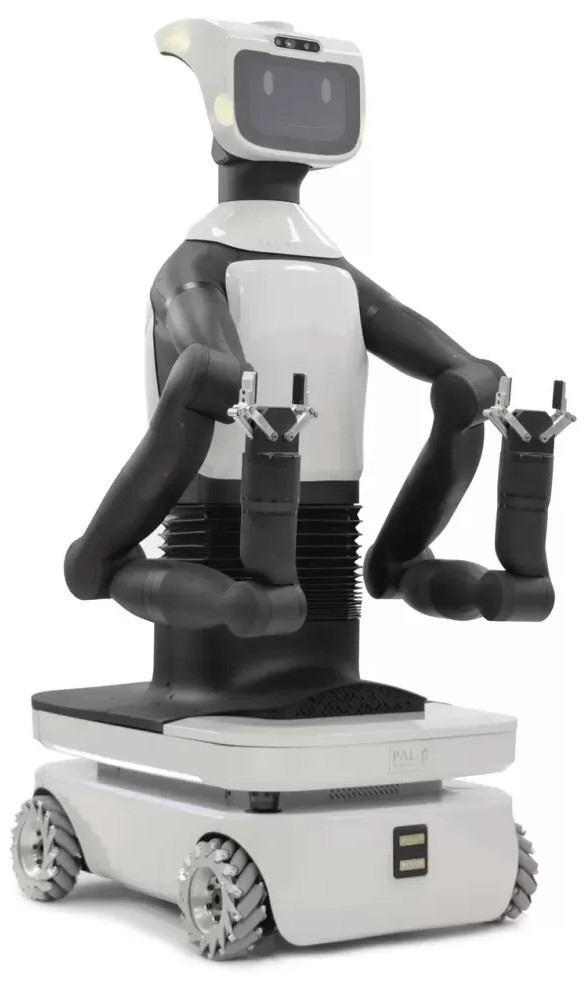
\includegraphics[width=\linewidth]{tiagopro}
    \label{fig:tiagopro}
\end{wrapfigure}


I will extract basic social descriptors using the ROS4HRI social perception
framework~\cite{lemaignan2022ros}, and is already available on robots like
TIAGo Pro. ROS4HRI provides information like the position, velocity, gaze
direction of every person in the vicinity of the robot. 

I will augment these basic descriptors with more complex percepts, including
(1) descriptors of human-objects interactions (HOI), using transformer-based
techniques like~\cite{iftekhar2022what}; (2) affective
descriptors~\cite{vinciarelli2009social}, using e.g. facial expressions based
on facial action units classification~\cite{martinez2019automatic}; (3)
group-level interactions, including $f$-formations~\cite{setti2015fformation},
and group activity recognition, using deep convolutional graph techniques like
ARG~\cite{wu2019learning}.

The TIAGoPro robot that I will acquire in \project is equipped with an on-board
GPU (NVidia Jetson family), that should provide the necessary compute resources
to run these algorithm in real-time on the robot itself. However, adding
additional compute resources could be easily achieved if necessary, since the
robot runs on the distributed ROS middleware, thus making it transparent to add
additional networked compute nodes.

\begin{framed}
    {\noindent\bf Main outcomes of \tCA:} lorem ipsum 
\end{framed}

\paragraph{\TCB}

\begin{rewrite}
Lorem ipsum dolor sit amet, consectetur adipiscing elit. Quisque non leo eu
lorem aliquet rutrum sed in ligula. Mauris sit amet orci quis nisl commodo
finibus tincidunt ac neque. Nam vel sem tempus, faucibus sapien eu,
imperdiet velit. Aenean ullamcorper finibus ipsum ut vestibulum. In dictum
suscipit tellus a volutpat. Duis pharetra lorem tristique vehicula volutpat.
Cras pellentesque, metus lacinia sagittis blandit, massa magna dignissim
elit, sed feugiat erat mauris tristique ipsum. Sed eget diam vitae magna
sollicitudin malesuada. Aenean vitae nisl ullamcorper, mattis ex sit amet,
convallis lorem. Donec maximus nec diam a fermentum. Quisque sed malesuada
nunc. Phasellus sagittis, erat feugiat sodales accumsan, libero libero
consectetur diam, vitae dignissim orci purus id enim.

Suspendisse vel felis hendrerit, elementum nunc imperdiet, semper massa. Cras id
sollicitudin massa. Etiam vel consequat eros. Fusce egestas placerat
pulvinar. Integer nulla ex, cursus vitae lobortis eget, congue at orci.
Donec non porttitor turpis, eu porttitor justo. Morbi non velit bibendum
mauris hendrerit efficitur. Proin malesuada sem at felis posuere, ac
tincidunt ligula hendrerit. Praesent non est vestibulum nunc commodo
tincidunt. Sed laoreet convallis augue eget ornare. Duis auctor nisi eu
egestas hendrerit. Ut porttitor gravida arcu, sed ornare metus scelerisque
sit amet. 
\end{rewrite}



\begin{framed}
    {\noindent\bf Main outcomes of \tCB:} lorem ipsum 
\end{framed}

\paragraph{\TCC}

Task \TCC is about designing and implementing a complete socio-cognitive
architecture for \project, by integrating in a principled way social embeddings
with the robot's decision-making mechanisms.

Developing a full cognitive architecture for service robots is beyond the scope
of the \project project. As such, this task will build on the extensive state
of art in cognitive architectures: disembodied
ones~\cite{chong2007integrated,vernon2007survey,kingdon2008review,duch2008cognitive,langley2009cognitive,taatgen2010past,thorisson2012cognitive},
as well as ones specifically developed for robotics like
ACT-R/E~\cite{trafton2013act}, HAMMER~\cite{demiris2006hierarchical}, KnowRob
2.0/CRAM~\cite{beetz2010cram, beetz2018knowrob},
POETICON++~\cite{antunes2016human}, and my own, the LAAS Architecture for
Social Interaction~\cite{lemaignan2017artificial}. This last one, in
particular, is already partially implemented on the TIAGoPro robot, and will
serve as the basis for this task.

While the results of WP2 should enable a range of new social capabilities for
the robot, their principled integration in a cognitive architecture is an open
research question, that will lay at the centre of research project of the PHD3
student. One current and promissing direction of research that would support
this integration can be found in the \emph{predictive processing}
framework~\cite{schillaci2016exploration} that reframes the traditional
perception--reasoning--action loop as a single inferential process, aiming at
both predicting future perceptions, and continously acting to minimizing
possible prediction errors. While until now this framework has mainly been
applied to simple control problems in robotics~\cite{ciria2021predictive}, it
could provide solid theoretical foundation for the integration of social embeddings in practical cognitive architectures for robot like~\cite{lemaignan2017artificial}.

\begin{framed}
\noindent {\bf Main outcomes of \tCC:} The principled integration of social
embeddings in a complete cognitive architecture, implemented on the
    TIAGoPro robot. This architecture enables the experimental task~\tDD and effectively demonstrates socio-cognitive skills in line with the criteria laid out in WP4.\TODO{check that we indeed define such criterias}
\end{framed}



%%%%%%%%%%%%%%%%%%%%%%%%%%%%%%%%%%%%%%%%%%%%%%%%%%%%%%%%%%%%%%%%%%%%%%%%%%%
\subsubsection{WP4: \textbf{\WPD}}

\begin{framed}
\noindent{\bf WP Timeframe:} Y1.5-Y4; {\bf Team:} all, but primarily PD1, PD3, PHD1, PHD3.
\end{framed}

\paragraph{\TDA}

\begin{rewrite}
Lorem ipsum dolor sit amet, consectetur adipiscing elit. Quisque non leo eu
lorem aliquet rutrum sed in ligula. Mauris sit amet orci quis nisl commodo
finibus tincidunt ac neque. Nam vel sem tempus, faucibus sapien eu,
imperdiet velit. Aenean ullamcorper finibus ipsum ut vestibulum. In dictum
suscipit tellus a volutpat. Duis pharetra lorem tristique vehicula volutpat.
Cras pellentesque, metus lacinia sagittis blandit, massa magna dignissim
elit, sed feugiat erat mauris tristique ipsum. Sed eget diam vitae magna
sollicitudin malesuada. Aenean vitae nisl ullamcorper, mattis ex sit amet,
convallis lorem. Donec maximus nec diam a fermentum. Quisque sed malesuada
nunc. Phasellus sagittis, erat feugiat sodales accumsan, libero libero
consectetur diam, vitae dignissim orci purus id enim.

Suspendisse vel felis hendrerit, elementum nunc imperdiet, semper massa. Cras id
sollicitudin massa. Etiam vel consequat eros. Fusce egestas placerat
pulvinar. Integer nulla ex, cursus vitae lobortis eget, congue at orci.
Donec non porttitor turpis, eu porttitor justo. Morbi non velit bibendum
mauris hendrerit efficitur. Proin malesuada sem at felis posuere, ac
tincidunt ligula hendrerit. Praesent non est vestibulum nunc commodo
tincidunt. Sed laoreet convallis augue eget ornare. Duis auctor nisi eu
egestas hendrerit. Ut porttitor gravida arcu, sed ornare metus scelerisque
sit amet. 
\end{rewrite}

\begin{framed}
    {\noindent\bf Main outcomes of \tDA:} lorem ipsum 
\end{framed}

\paragraph{\TDB}

The social situation awareness capabilities enabled by the use of social embedding will be
demonstrated through a series of studies:

\begin{itemize}
    \item {\bf situational awareness (SA)}: situational
        awareness~\cite{endsley1995theory} is a precursor of social situation
        awareness. This first study will evidence how social embeddings directly
        enable to implement it. Instead of relying on the standard SAGAT test of
        SA~\cite{endsley2017direct}, I will use a protocol proposed by Dahn et
        al. in~\cite{dahn2018situation}, specifically designed for robots, and
        based on the ability for a robot to recognise an event as being
        unexpected. This protocol has the advantage of being directly adaptable
        to social embeddings.

    \item {\bf social intelligence quotient (SQ)} is the generic name for tests
        of social intelligence. While these tests have existed for a long time
        (e.g.~\cite{moss1930social}), I will adapt to robots more recent and shorter tests
        (short form of the Reading the Mind in the Eyes
        test~\cite{olderbak2015psychometric}) to show and measure how contextualized social
        embeddings can endow robot with a level of social intelligence (and not
        only elicit the \emph{perception} of social intelligence, like in
        e.g.~\cite{barchard2020measuring}.

    \item I will also adapt to social robotics~\cite{lemaignan2015mutual}
        experimental protocols originally designed by Frith and
        Happé~\cite{frith1994autism} to investigate social representation and
        mental modelling in autistic children.  This protocol include tasks like
        distinguishing \emph{happiness} or \emph{sadness} from \emph{surprise},
        or distinguishing \emph{sabotage} from \emph{deception}: these nuances,
        quite self-explanatory to experienced social agents, require subtle
        modelling of the context and mental state of agents, and, until now,
        have not been successfully reproduced on robots. I aim to show that
        social embeddings offer a generic methodology to implement this kind of
        advanced social situation awareness.

\end{itemize}

\begin{framed}
    {\noindent\bf Main outcomes of \tDB:} lorem ipsum 
\end{framed}

\paragraph{\TDC}

\begin{rewrite}
Lorem ipsum dolor sit amet, consectetur adipiscing elit. Quisque non leo eu
lorem aliquet rutrum sed in ligula. Mauris sit amet orci quis nisl commodo
finibus tincidunt ac neque. Nam vel sem tempus, faucibus sapien eu,
imperdiet velit. Aenean ullamcorper finibus ipsum ut vestibulum. In dictum
suscipit tellus a volutpat. Duis pharetra lorem tristique vehicula volutpat.
Cras pellentesque, metus lacinia sagittis blandit, massa magna dignissim
elit, sed feugiat erat mauris tristique ipsum. Sed eget diam vitae magna
sollicitudin malesuada. Aenean vitae nisl ullamcorper, mattis ex sit amet,
convallis lorem. Donec maximus nec diam a fermentum. Quisque sed malesuada
nunc. Phasellus sagittis, erat feugiat sodales accumsan, libero libero
consectetur diam, vitae dignissim orci purus id enim.

Suspendisse vel felis hendrerit, elementum nunc imperdiet, semper massa. Cras id
sollicitudin massa. Etiam vel consequat eros. Fusce egestas placerat
pulvinar. Integer nulla ex, cursus vitae lobortis eget, congue at orci.
Donec non porttitor turpis, eu porttitor justo. Morbi non velit bibendum
mauris hendrerit efficitur. Proin malesuada sem at felis posuere, ac
tincidunt ligula hendrerit. Praesent non est vestibulum nunc commodo
tincidunt. Sed laoreet convallis augue eget ornare. Duis auctor nisi eu
egestas hendrerit. Ut porttitor gravida arcu, sed ornare metus scelerisque
sit amet. 
\end{rewrite}


\begin{framed}
    {\noindent\bf Main outcomes of \tDC:} lorem ipsum 
\end{framed}


\paragraph{\TDD}

\begin{rewrite}
Lorem ipsum dolor sit amet, consectetur adipiscing elit. Quisque non leo eu
lorem aliquet rutrum sed in ligula. Mauris sit amet orci quis nisl commodo
finibus tincidunt ac neque. Nam vel sem tempus, faucibus sapien eu,
imperdiet velit. Aenean ullamcorper finibus ipsum ut vestibulum. In dictum
suscipit tellus a volutpat. Duis pharetra lorem tristique vehicula volutpat.
Cras pellentesque, metus lacinia sagittis blandit, massa magna dignissim
elit, sed feugiat erat mauris tristique ipsum. Sed eget diam vitae magna
sollicitudin malesuada. Aenean vitae nisl ullamcorper, mattis ex sit amet,
convallis lorem. Donec maximus nec diam a fermentum. Quisque sed malesuada
nunc. Phasellus sagittis, erat feugiat sodales accumsan, libero libero
consectetur diam, vitae dignissim orci purus id enim.

Suspendisse vel felis hendrerit, elementum nunc imperdiet, semper massa. Cras id
sollicitudin massa. Etiam vel consequat eros. Fusce egestas placerat
pulvinar. Integer nulla ex, cursus vitae lobortis eget, congue at orci.
Donec non porttitor turpis, eu porttitor justo. Morbi non velit bibendum
mauris hendrerit efficitur. Proin malesuada sem at felis posuere, ac
tincidunt ligula hendrerit. Praesent non est vestibulum nunc commodo
tincidunt. Sed laoreet convallis augue eget ornare. Duis auctor nisi eu
egestas hendrerit. Ut porttitor gravida arcu, sed ornare metus scelerisque
sit amet. 
\end{rewrite}


\begin{framed}
    {\noindent\bf Main outcomes of \tDD:} lorem ipsum 
\end{framed}



%%%%%%%%%%%%%%%%%%%%%%%%%%%%%%%%%%%%%%%%%%%%%%%%%%%%%%%%%%%%%%%%%%%%%%%%%%%
\subsubsection{WP5: \textbf{\WPZ}}

\begin{framed}
\noindent{\bf WP Timeframe:} Y1-Y5; {\bf Team:} all
\end{framed}

The last workpackage groups all the task related to the grant management, as
well as the dissemination and exploitation tasks.

The interdiscplinary nature of the project means that dissemination actions, in
particular, needs to target a broader range of practionners and stakeholders
than in typical projects.

\project has the ambition to disrupt how we study social interactions. While
the experimental side of the project is focused on applications in social
robotics, the impact of the project is not limited to this field, and I intend
to disseminate this work to a range of academic communities, from pure AI, to
the emerging field of data-driven sociology.

\TODO{how specific about dissemination/exploitation actions?}

\paragraph{\TZA}

lorem ipsum

\begin{framed}
    {\noindent\bf Main outcomes of \tZA:} lorem ipsum 
\end{framed}

\paragraph{\TZB}

lorem ipsum

\begin{framed}
    {\noindent\bf Main outcomes of \tZB:} lorem ipsum 
\end{framed}

\paragraph{\TZC}

lorem ipsum

\begin{framed}
    {\noindent\bf Main outcomes of \tZC:} lorem ipsum 
\end{framed}




%%%%%%%%%%%%%%%%%%%%%%%%%%%%%%%%%%%%%%%%%%%%%%%%%%%%%%%%%%%%%%%%%%%%%%%%%%%
%%%%%%%%%%%%%%%%%%%%%%%%%%%%%%%%%%%%%%%%%%%%%%%%%%%%%%%%%%%%%%%%%%%%%%%%%%%
%%%%%%%%%%%%%%%%%%%%%%%%%%%%%%%%%%%%%%%%%%%%%%%%%%%%%%%%%%%%%%%%%%%%%%%%%%%
\subsection{Measures for a Responsible Robotics research}


Because the development of socially-intelligent robots has
complex ethical ramifications -- including the potential of alienating
human users, \project also includes an explicit research component on
Responsible Robotics. In particular, the project will aim to contribute directly
to the on-going roadmap for Responsible Robotics, specifically
investigating the interplay between social embeddings, transparency and human
agency. The work will be conducted in workpackage WP4.


Social embeddings, by enabling artificial systems to model and reason on their
social environment, have the potential of significantly increase the social
competencies of e.g. robots, also raising ethical questions.

\begin{rewrite}
I am part of an international working group on Responsible Robotics~\TODO{cite
Dagsthul roadmap arxiv}...

%WP6 aims at establishing the conceptual and ethical framework around the idea of
%\emph{robot-supported human-human interactions}. It does so by co-creating
%patterns of interaction and norms with the general public, using a unique
%combination of ethnographic observations and `crowd-sourced' interaction
%patterns.
%
%\vspace{1em}
%\noindent\emph{Timeframe: Y3-Y5; one senior post-doc (PD3)
%with background in ethics of technology and responsible innovation.}





%
%\subsubsection{Background on social robotic ethics}\label{ethics}
%
%The ethical questions raised by social robotics have been actively studied over
%the last 5 years, attempting to address issues like:
%
%\begin{itemize}
%    \item how to ensure that social robots are not used to simply replace the human
%        workforce to cut costs?
%    \item can we provide guarantees that the use of social robots will always be
%        ethically motivated?
%    \item further on, can we implement some ethical safeguarding built-in
%        the system (like an ethical \emph{black-box}~\cite{winfield2017case})?
%    \item what about privacy? how to trust robots in our home or school or
%        hospital not to eavesdrop on our private lives, and, in the worst
%        case, not be used \emph{against} us?
%\end{itemize}
%
%These questions are indeed pressing. The recent rise of personal assistants like
%Amazon Alexa or Google Home, with the major privacy concerns that accompanies
%their deployments in people home, shows that letting the industry set the agenda
%on these questions is not entirely wise -- and robots can potentially be much
%more intrusive than non-mobile smart speakers.  The EU is positioning itself at
%the forefront of those questions. The recent release of operational \textbf{Ethics
%Guidelines for Trustworthy AI} by the EU High-level Expert Group on Artificial
%Intelligence~\cite{eu2019ethics} is a strong sign of this commitment. These
%guidelines identify seven requirements of trustworthy AI:
%
%\begin{enumerate}[label=\textbf{R\arabic*}]
%    \item \textbf{Human agency and oversight}, including
%            fundamental rights, human agency and human oversight
%
%    \item \textbf{Technical robustness and safety}, including resilience to
%        attack and security, fall back plan and general safety, accuracy,
%        reliability and reproducibility
%
%    \item \textbf{Privacy and data governance}, including respect for privacy,
%        quality and integrity of data, and access to data
%
%    \item \textbf{Transparency}, including traceability, explainability and
%        communication
%
%    \item \textbf{Diversity, non-discrimination and fairness}, including the
%        avoidance of unfair bias, accessibility and universal design, and
%        stakeholder participation
%
%    \item \textbf{Societal and environmental wellbeing}, including
%        sustainability and environmental friendliness, social impact, society
%        and democracy
%
%    \item \textbf{Accountability}, including auditability, minimisation and
%        reporting of negative impact, trade-offs and redress.
%
%\end{enumerate}
%
%The design methodologies and techniques employed in \project naturally implement
%most of these requirements: interaction co-design and human-in-the-loop machine
%learning ensures human agency oversight over the robot's behaviours (R1);
%Privacy and data governance (R3) is addressed in the project's data management
%plan and facilitated by the design decision of performing all data processing
%on-board the robot, avoiding the dissemination of personal information; the
%transparency of the robot behaviour (R4) stems from the machine learning
%approach that we advocate: the robot's behaviours primarily originate from what
%the end-users themselves taught the robot; diversity and non-discrimination (R5)
%is supported by the large-scale involvement of the public at the science centre,
%ensuring a broad diversity of backgrounds and profiles; societal wellbeing (R6)
%is the core research question of the project, and \project will contribute in
%realising this requirement in the context of social robots.
%
%Technical robustness (R2) and accountability (R7) are important design
%guidelines for the robot's cognitive architecture (WP4), and will be addressed
%there as well.
%
%
%The Ethics Guidelines for Trustworthy AI form a solid foundation for the
%project. However, personal and social robots raise additional questions
%regarding what ethical and trustworthy systems might look like, and while the
%principles of responsible design are somewhat established~\cite{stahl2016ethics,
%bsi2016robots}, the reality of robot-influenced social interactions is not
%fully understood yet, if only because the technology required to experience such
%interactions is only slowly maturing. 
%
%Social robots have indeed two properties that stand out, and distinguish them
%from smart speakers, for instance.  First, they are fully embodied, and they
%physically interact with their environment, from moving around, to picking up
%objects, to looking at you; second, willingly or not, they are ascribed
%\emph{agency} by people. This second difference has far-reaching consequences,
%from affective bonding to over-trust, to over-disclosure of personal, possibly
%sensitive, informations~\cite{martelaro2016tell,shiomi2017robot}.  As an
%example, a common objection to human-robot interaction is the perceived
%deceptive nature of the robot's role. It has been
%argued~\cite{biscontilucidi2018companion} that the underlying concern is likely
%the lack of an adequate (and novel) model of human-robot interactions to refer
%to, to which the project will provide elements of response. This needs
%nevertheless to be accounted for in depth.
%
%Ethical framing of social robotics has started to
%emerge under the term \textbf{roboethics}: the ``subfield of applied ethics
%studying both the positive and negative implications of robotics for individuals
%and society, with a view to inspire the moral design, development and use of
%so-called intelligent/autonomous robots, and help prevent their misuse against
%humankind.''~\cite{allen2011robot}. Specific subfields, like assistive
%robotics~\cite{sharkey2012granny}, have seen some additional work, but social
%robotics is still not equipped with operational guidelines, similar to the EU
%guidelines on trustworthy AI.
%
%\subsubsection{\project-specific measures}
%
%I have chosen to focus the first workpackage task (T1.1) on building an
%operational ethical framework for social robots which engage over long period of
%time with the public. This work will deliver initial guidelines -- strongly
%inspired by the guidelines on Trustworthy AI -- that will both form the ethics
%basis for the \project experimental fieldwork, and have an impact beyond the
%project, to feed into future European-level guidelines.
%
%This work will be supported by an Ethics Advisory Board, composed of 3 experts
%in ethics and social robotics and AI. While the exact composition of the board
%is not final yet, it will include at least one member from the EU High-Level
%Expert Group on Artificial Intelligence, that will be able to share the EU
%expertise in framing ethics guidelines.
%
%Practically speaking, these guidelines will form the basis of the ethics
%approval process for the three long-term \project studies. It will be
%additionally supported by my extensive experience in seeking ethics approval for
%studies involving robots and vulnerable populations (in particular,
%children~\cite{lemaignan2016learning,lemaignan2018pinsoro,senft2019teaching}),
%the expertise of Dr. Newbutt in conducting research with SEN schools (O2.1.1), and
%the support of J. Bowyer at the Bristol's Children's Hospital to obtain NHS ethics
%approval. \textbf{As per requested, details of the ethics approval process,
%children safeguarding, research Code of Conduct, and Data Management Plan are
%annexed to the project proposal, in a separate `Ethics and Data Protection'
%document}.
%
%The project will also follow the European Commission recommendations for
%Responsible Research and Innovation (RRI). RRI is defined
%in~\cite{stilgoe2013developing} (and has been subsequently adopted by the UK Engineering
%and Physical Sciences Research Council~\cite{owen2014uk}) using the acronym
%AREA: Anticipation, Reflection, Engagement and Action. The \project research
%will be undertaken responsibly by (1) \ul{Anticipating} possible consequences;
%(2) by integrating mechanisms of \ul{Reflection} about the conducted work and its
%aims; (3) by \ul{Engaging} with relevant stakeholders (general public, teachers,
%hospital staff, parents, children themselves); and (4) by \ul{Guiding} action of
%researchers accordingly. This approach has been formalised in the AREA 4P
%framework~\cite{stahl2018implementing}~\footnote{\url{https://www.orbit-rri.org/about/area-4p-framework/}},
%that I will use to guide the research strategy over the course of the project.
%An additional role of the Ethics Advisory Board will be to advise and audit the
%project with regards to this framework for responsible research.
%
\end{rewrite}



%%%%%%%%%%%%%%%%%%%%%%%%%%%%%%%%%%%%%%%%%%%%%%%%%%%%%%%%%%%%%%%%%%%%%%%%%%%
\subsection{Risk/gain analysis}

\TODO{how much of that do we need?}

\begin{rewrite}

\textbf{Tasks 1.1, 1.2} develop a novel methodology, `public-in-the-loop' machine
learning, for large-scale co-design of social interactions with the public. If
successful, this will be of great value, well beyond the project. The
proposed experimental setup (science centre visitors `taking control' of the robot)
might however lead to interactions that are either too short or to artificial to
create meaningful, generalisable social interaction. In addition, the messy and
complex nature of the science centre environment is also currently beyond-state-of-the-art
in term of extracting the useful social features required to train a classifier.

However, the interaction principles that we want to uncover in T1.1 and T1.2
(and that are feeding into WP2 and WP4) will principally come from a qualitative
analysis of the interactions, carried in parallel to the machine learning
approach. This well within the expertise of the PI, and, as such, is low-risk.
T1.1 can thus be described as a \ul{\bf medium-risk, high-gain} component of
\project.

\vspace{1em}

\textbf{Task 2.1} develops a novel situation assessment component, that
integrates spatio-temporal modeling with knowledge representation. The resulting
component is beyond-state-of-the-art, and would be highly relevant to a large range
of robotic applications. This component relies on integrating tools that are
independently relatively mature and well understood, and the principles of the
integration itself is already well researched. Besides, it falls well within the
PI
expertise~\cite{lemaignan2018underworlds,sallami2019simulation,lemaignan2010oro}.
As such, O2.2.1 can be described as \ul{\bf low-risk, medium-gain}.

\textbf{Tasks 2.2, 2.3, 2.4} Work on real-time modeling of social dynamics in
real-world environments are only begining to be studied in robotics. While the
underpinning are well understood in neighbouring academic fields, a very
significant work remain to be done to integrate disparate or partial approaches
into one framework. These tasks also require the acquisition of novel datasets
that focus on natural human-human social interactions. The PI has extensive
experience in building and acquiring such
datasets~\cite{lemaignan2018pinsoro,sallami2020unexpected}, and does not
foreseen major difficulties. The resulting components have however the potential
to unlock a new class of social robots, aware in real-time of their social
surroundings and dynamics.  These tasks are thus considered \ul{\bf low-risk,
high-gain}.

\vspace{1em}

\textbf{Task 3.1} The behavioural baseline implements the current state-of-the-art,
and as such is \ul{\bf low-risk, low-gain}. T3.1 will guarantee early on in the
project a `working' robot, yet with predictable/repetitive behaviours.

\textbf{Task 3.2} The neural generation of complex social behaviours is a
\ul{\bf medium-risk, high-gain} task: while it builds on solid existing
state-of-the-art, it relies on very significant progress in both the modeling of the
social dynamics (WP2) and the capacity of designing a machine learning approach
to learn and generate these complex behaviours. While the former falls well
within the PI expertise, machine learning for social motion generation is
essentially a novel field. The success of this task will rely to a large
extend on the quality of the post-doctoral researcher recruited to lead this
effort. The main mitigation to the risk associated to T3.2 is the behavioural
baseline created in T3.1: the behavioural capabilities generated in T3.2 can be
complemented by ad-hoc behaviours whenever required.

\textbf{Task 3.3} Non-verbal communication is a well established subfield of HRI
research, well known to the PI. The creation of the novel interaction modality
based on soundscape is novel, with potential for impact beyond the project. This
new modality will be co-developped with an expert of sound design for
interaction, and we do not foresee major risks. Overall, the task is \ul{\bf
low-risk, medium-gain}.

\vspace{1em}

\textbf{Task 3.1} The conceptual framing of a \emph{socially-driven
architecture} (social teleology) and its translation into decision-making
algorithms are to a large extend open questions. This task might however lead to
uncover a fundamental mechanism to enable long-term engagement of users
with social robots. Building fundamentally on blue-sky research, this task is
\ul{\bf high-risk, high-gain}. If not successful, I will instead rely on the
decision-making strategy of T3.2, which is much lower risk.

\textbf{Task 3.2} The techniques developed in T3.2 have been previously used and
tested by the PI in two different real-world
environments~\cite{senft2019teaching,winkle2020couch}. While they will require
significant adjustments for this project, the task is overall \ul{\bf low-risk,
low-gain}.

\textbf{Task 3.3} The integration of the different cognitive functions of the
robot into one principled cognitive architecture, that include cognitive
redundancy, is one of the core expertise of the
PI~\cite{lemaignan2017artificial}. This task however includes significant novel
elements (cognitive mechanisms for long-term autonomy; decision arbitration)
that bear unknowns. Besides, this task is a critical pre-requisite for WP5. As a
result, T3.3 is considered as \ul{\bf high-risk}. The task is focused on
integration to meet the requirements of the WP5 experiments, and parts
of the resulting software architecture might be project-specific. However the
overall aims of endowing the robot with long-term social autonomy would be a
significant breakthrough, and as such, T3.3 is \ul{\bf high-gain}. The main
mitigations comes from (1) the iterative development process of the
architecture, that will start from the existing state-of-the-art, to which the
PI has previously contributed~\cite{lemaignan2017artificial}. By doing so, a
decisional architecture for the robot will be available early on in the project.
While that architecture might be a scaled-down version of the initial ambition,
it will still enable the fieldwork proposed in WP5, possibly with a lesser level
of autonomy; (2) the possibility of using only one of the two action policies
(T3.1 \ul{or} T3.2), thus removing the need for complex arbitration.

\vspace{1em}

\textbf{WP5: Experimental deployments}

The two application scenarios (at the children hospital and in the SEN school)
are ambitious and inherently risky, as they target vulnerable populations.
However, first, demonstrating the importance of advanced social modelling, and
convincingly proving the effectiveness of our approach does require accordingly
complex social situations, and complex social dynamics. The two scenarios, which
complement each other, provide both.

Second, working with vulnerable populations, in constrained and complex
environments (children hospital and SEN schools) adds significant risks to the
project. But it is also what make the project in the unique position of
delivering a high societal impact: a direct positive impact on children's lives
(we anticipate 100+ hospitalised children and 50+ children with psycho-social
impairements interacting over long periods of time with a robot over the course
of the project), and a broader impact on the society, showing how robots can
have a lasting, strong, positive impact on the society, also establishing the
idea of \emph{robots supporting human interactions} instead of dehumanising our
social relationships.

\textbf{Together, Task 5.1 and 5.2 are \ul{high-risk, high-gain}.}

The two main mitigations are (1) early and continuous engagement with the
stakeholders, and (2) the decoupling of the two applications, meaning that the
risks associated to each of them do not impact the other one.

Early engagement will be ensured by relying on a participatory design
methodology, involving all the stakeholders from the onset of the project; the
methodology will involve regular joint workshops; on-site (hospital and SEN
schools) research stay including engagement with the staff/charities and the
children themselves; early field testing and prototyping, relying if necessary
on provisional, yet well-known, robot platforms available at the host
institution (for instance, Softbank Nao and Pepper). This user-centered approach
will be championed by the post-doc recruited on the project on WP4 and WP5, who will
have to have a strong expertise in user-centered design.

It is also important to note that, while preparing this bid, initial discussions
have been held with all the partners involved with the experimental fieldwork
(WeTheCurious science centre, Bristol's Children Hospital, the network of SEN
schools): each of these institutions is enthusiastic about the project, already
contributing ideas to integrate the robots in their daily routines, and
ready to dedicate time and effort for its success.


\end{rewrite}




%%%%%%%%%%%%%%%%%%%%%%%%%%%%%%%%%%%%%%%%%%%%%%%%%%%%%%%%%%%%%%%%%%%%%%%%%%%
\newpage
\printbibliography



\newpage

%%%%%%%%%%%%%%%%%%%%%%%%%%%%%%%%%%%%%%%%%%%%%%%%%%%%%%%%%%%%%%%%%%%%%%%%%%%%%
%%%%%%%%%%%%%%%%%%%%%%%%%%%%%%%%%%%%%%%%%%%%%%%%%%%%%%%%%%%%%%%%%%%%%%%%%%%%%
%%%%%%%%%%%%%%%%%%%%%%%%%%%%%%%%%%%%%%%%%%%%%%%%%%%%%%%%%%%%%%%%%%%%%%%%%%%%%

\chapter{Appendix: Current research grants and any on-going applications related
to the proposal}

\TODO{to update}
\subsection{Current Grants}

\begin{tabular}{p{1.8cm}p{1.8cm}llp{4cm}p{4cm}}
\toprule
\textbf{Project Title} & \textbf{Funding source} & \textbf{Amount} & \textbf{Period} & \textbf{Role of the PI} & \textbf{Relation to current  ERC proposal} \\ \midrule
    CoreSense & EU H2020 & &  & & \\ \midrule
    SPRING & EU H2020 & &  & & \\ \midrule
    TALBOT & EU H2020 & &  & & \\ \midrule
    SHAPES & EU H2020 & &  & & \\ \midrule
    PERSEO & EU H2020 & &  & & \\ \midrule
\end{tabular}

\subsection{On-going and submitted grant applications}

\begin{tabular}{p{1.8cm}p{1.8cm}llp{4cm}p{4cm}}
\toprule
\textbf{Project Title} & \textbf{Funding source} & \textbf{Amount} & \textbf{Period} & \textbf{Role of the PI} & \textbf{Relation to current  ERC proposal} \\ \midrule
    ... & & &  & & \\ \midrule
\end{tabular}



\end{document}
